% !TEX root = thesis.tex
\documentclass[12pt,a4paper,titlepage,listof=totoc,bibliography=totoc,chapteratlists=0pt]{scrreprt}
\newcommand{\thesislang}{en} % en or de
\newcommand{\thesistitle}{Kipper - Programming Language for Improved Runtime Type-Safety}
\newcommand{\department}{Higher Department of Informatics} % Replace with your department

\newcommand{\firstauthor}{Luna Klatzer}
\newcommand{\secondauthor}{Lorenz Holzbauer}
\newcommand{\thirdauthor}{Fabian Baitura}

\newcommand{\duedateen}{April 4, 2025} % due date in English format
\newcommand{\duedatede}{4. April 2025} % due date in German format
\newcommand{\supervisor}{Peter Bauer}
\newcommand{\projectpartner}{Dr. Hanspeter Mössenböck, Johannes Kepler University}

\begin{filecontents*}{\jobname.xmpdata}
	\Keywords{Compiler, Transpiler, Programming Language, Type-Safety, Node, JKU}
	\Title{Kipper - Programming Language for Improved Runtime Type-Safety}
	\Author{Luna Klatzer, Lorenz Holzbauer, Fabian Baitura}
\end{filecontents*}

\setcounter{tocdepth}{2}

\usepackage[utf8]{inputenc}
\usepackage[T1]{fontenc}
\usepackage{amsmath}
\usepackage{amsfonts}
\usepackage{amssymb}
\usepackage[table]{xcolor}
\usepackage{graphicx}
\usepackage[left=3.50cm, right=2.00cm, top=2.00cm, bottom=2.00cm,foot=1cm]{geometry}
\usepackage[splitrule,hang,flushmargin,multiple,bottom]{footmisc}
\usepackage{lmodern, textcomp}
\usepackage{lmodern}
\usepackage{pdfpages}
\usepackage[german, english]{babel}
\usepackage{multicol}
\usepackage{float}
\usepackage{array,tabularx,booktabs}
\usepackage{ragged2e}
\usepackage{lipsum}
\usepackage{wrapfig}
\usepackage{stackengine}
\usepackage[export]{adjustbox}

\newcolumntype{M}[1]{>{\centering\arraybackslash}m{#1}}
\scriptsize
\usepackage{enumitem}
\newlist{compactitem}{itemize}{3}
\setlist[compactitem,1]{label=\textbullet, nosep,leftmargin=1.5em,labelwidth=*,align=left}
\setlist[compactitem,2]{label=--, nosep,leftmargin=1.5em,labelwidth=*,align=left}
\setlist[compactitem,3]{label=\textopenbullet, nosep,leftmargin=1.5em,labelwidth=*,align=left}
\newlist{compactenum}{enumerate}{3}
\setlist[compactenum,1]{label=\arabic*., nosep,leftmargin=1.5em,labelwidth=*,align=left}
\setlist[compactenum,2]{label=\alph*., nosep,leftmargin=1.5em,labelwidth=*,align=left}
\setlist[compactenum,3]{label=\roman*., nosep,leftmargin=1.5em,labelwidth=*,align=left}
\newlist{compactdesc}{description}{3}
\setlist[compactdesc]{leftmargin=1.5em,labelwidth=*,align=left}

\usepackage{microtype}

\usepackage[parfill]{parskip}

\definecolor{bluekeywords}{rgb}{0.13,0.13,1}
\definecolor{greencomments}{rgb}{0,0.5,0}
\definecolor{redstrings}{rgb}{0.9,0,0}
\definecolor{lightgray}{gray}{0.9}
\definecolor{lightblue}{rgb}{0.93,0.95,1.0}

\usepackage{listings}

\makeatletter
\lstdefinestyle{lststyle}{
	basicstyle=%
	\ttfamily
	\lst@ifdisplaystyle\scriptsize\fi
}
\makeatother

\renewcommand{\lstlistlistingname}{List of Listings}
\lstset{
morekeywords={base,var,in,out,dynamic,from,where,select,orderby,function,\$,group,by,into,yield,async,await,@,None,self,as,elif,with}
}
\lstdefinelanguage{JavaScript}{
	morekeywords={typeof, new, true, false, catch, function, return, null, switch, var, if, in, while, do, else, case, break, void, module, \$, export, for, this, class, extends, constructor, var, let, const, super, null, undefined},
	keywordstyle=\color{blue}\bfseries,
	morekeywords=[2]{class, export, boolean, throw, implements, import, this},
	keywordstyle=[2]\color{darkgray}\bfseries,
	sensitive=true,
	morecomment=[l]{//},           % Line comments
	morecomment=[s]{/*}{*/},       % Block comments
	commentstyle=\color{gray}\itshape,
	morestring=[b]',               % Strings enclosed in single quotes
	morestring=[b]",               % Strings enclosed in double quotes
	stringstyle=\color{green!50!black},
	identifierstyle=\color{black},
	basicstyle=\ttfamily\normalsize,
	captionpos=b,
	frame=single,
	framesep=4pt,
	framerule=0.5pt,
	framextopmargin=6pt
}

\lstdefinelanguage{TypeScript}{
	morekeywords={typeof, new, true, false, catch, function, return, null, switch, var, if, in, while, do, else, case, break, void, module, \$, export, for, this, class, interface, enum, extends, implements, constructor, var, let, const, super, null, undefined, number, string, boolean, object, bigint, symbol},
	keywordstyle=\color{blue}\bfseries,
	morekeywords=[2]{class, export, boolean, throw, implements, import, this},
	keywordstyle=[2]\color{darkgray}\bfseries,
	sensitive=true,
	morecomment=[l]{//},           % Line comments
	morecomment=[s]{/*}{*/},       % Block comments
	commentstyle=\color{gray}\itshape,
	morestring=[b]',               % Strings enclosed in single quotes
	morestring=[b]",               % Strings enclosed in double quotes
	stringstyle=\color{green!50!black},
	identifierstyle=\color{black},
	basicstyle=\ttfamily\normalsize,
	captionpos=b,
	frame=single,
	framesep=4pt,
	framerule=0.5pt,
	framextopmargin=6pt
}
\lstdefinelanguage{Rust}{
	morekeywords={
		as, break, const, continue, crate, else, enum, extern, false, fn, for, if, impl, in, let, loop, match, mod, move, mut, pub, ref, return, self, Self, static, struct, super, trait, true, type, unsafe, use, where, while, async, await, dyn
	},
	morekeywords=[2]{abstract, become, box, do, final, macro, override, priv, try, typeof, unsized, virtual, yield},
	sensitive=true,
	morestring=[b]{"}, % Strings enclosed in double quotes
	morestring=[b]{'}, % Strings enclosed in single quotes
	morecomment=[l]{//}, % Line comments
	morecomment=[s]{/*}{*/}, % Block comments
	keywordstyle=\color{blue}\bfseries,
	sensitive=true,
	commentstyle=\color{gray}\itshape,
	stringstyle=\color{green!50!black},
	identifierstyle=\color{black},
	basicstyle=\ttfamily\normalsize,
	captionpos=b,
	frame=single,
	framesep=4pt,
	framerule=0.5pt,
	framextopmargin=6pt
}
\lstdefinelanguage{Antlr4}{
	morekeywords={grammar,parser,lexer,options,returns,locals,throws,catch,finally,
		import,tokens,channel,skip,fragment,protected,public,private},
	sensitive=true,
	morestring=[b]{"}, % Strings enclosed in double quotes
	morestring=[b]{'}, % Strings enclosed in single quotes
	morecomment=[l]{//}, % Line comments
	morecomment=[s]{/*}{*/}, % Block comments
	keywordstyle=\color{blue}\bfseries,
	sensitive=true,
	commentstyle=\color{gray}\itshape,
	stringstyle=\color{green!50!black},
	identifierstyle=\color{black},
	basicstyle=\ttfamily\normalsize,
	captionpos=b,
	frame=single,
	framesep=4pt,
	framerule=0.5pt,
	framextopmargin=6pt
}
\lstset{
	language=TypeScript,
	numbers=left,
	numberstyle=\scriptsize,
	showspaces=false,
	showtabs=false,
	breaklines=true,
	lineskip=-1pt,
	tabsize=2,
	showstringspaces=false,
	breakatwhitespace=true,
	escapeinside={(*@}{@*)},
	commentstyle=\color{greencomments},
	keywordstyle=\color{bluekeywords}\bfseries,
	stringstyle=\color{redstrings},
	style=lststyle,
	xleftmargin=17pt,
	framexleftmargin=17pt,
	framexrightmargin=5pt,
	framexbottommargin=4pt,
	basicstyle=\ttfamily\normalsize,
	captionpos=b,
	frame=single,
	framesep=4pt,
	framerule=0.5pt,
	framextopmargin=6pt
}

\usepackage{caption}
\DeclareCaptionFont{white}{\color{white}}
\DeclareCaptionFormat{listing}{\colorbox[cmyk]{0.43, 0.35, 0.35,0.01}{\parbox{\textwidth}{\hspace{10pt}#1#2#3}}}
\captionsetup[lstlisting]{format=listing,labelfont=white,textfont=white}
\captionsetup[table]{justification=centering, singlelinecheck=false}

\usepackage{subcaption}

\usepackage{setspace}
\newcommand{\MSonehalfspacing}{%
	\setstretch{1.44}%  default
	\ifcase \@ptsize \relax % 10pt
	\setstretch {1.448}%
	\or % 11pt
	\setstretch {1.399}%
	\or % 12pt
	\setstretch {1.433}%
	\fi
}

\newcommand{\setauthor}[1]{\ohead[]{#1}}

\usepackage[automark]{scrlayer-scrpage}
\pagestyle{scrheadings}
\automark{chapter}
\renewcommand\sectionmark[1]{\markright{\MakeMarkcase {\thesection\hskip .5em\relax#1}}}
\rohead{\ifnum\expandafter\pdfstrcmp\botmark=0 \rightmark\else\leftmark{} --- \rightmark\fi}
\ihead[]{\headmark}
\chead[]{}
\ohead{}
\cfoot[]{}
\ofoot[\pagemark]{\pagemark}
\setheadsepline{.1pt}

\usepackage[hyphens]{url}

\usepackage[a-1b]{pdfx}

\usepackage{hyperref}
\hypersetup{pdfa}

\usepackage[nonumberlist,toc,nopostdot,acronym]{glossaries}

\usepackage{chngcntr}
\counterwithout{footnote}{chapter}
\counterwithout{figure}{chapter}
\counterwithout{table}{chapter}
\AtBeginDocument{
	\counterwithout{lstlisting}{chapter}
	\urlstyle{sf}
}
\newcounter{RPages}

\selectlanguage{english}

\makeatletter
\def\bstctlcite{\@ifnextchar[{\@bstctlcite}{\@bstctlcite[@auxout]}}
\def\@bstctlcite[#1]#2{\@bsphack
	\@for\@citeb:=#2\do{%
		\edef\@citeb{\expandafter\@firstofone\@citeb}%
		\if@filesw\immediate\write\csname #1\endcsname{\string\citation{\@citeb}}\fi}%
	\@esphack}
\makeatother

\clubpenalty=10000 
\widowpenalty=10000
\displaywidowpenalty=10000
\interfootnotelinepenalty=10000

\title{Kipper - Programming Language for Improved Runtime Type-Safety}
\author{Luna Klatzer, Lorenz Holzbauer, Fabian Baitura}

\makeindex
\makeglossaries
\begin{document}
\bstctlcite{IEEEexample:BSTcontrol}
\newcommand{\reminder}[1]
{ \textcolor{red}{<[{\bf\marginpar{\mbox{$<==$}} #1 }]>} }
\newcommand{\icode}[1]{\lstinline$#1$}
%\urlstyle{same}
%\setstretch{1.5}
\setstretch {1.433}
\renewcommand{\arraystretch}{1.2}

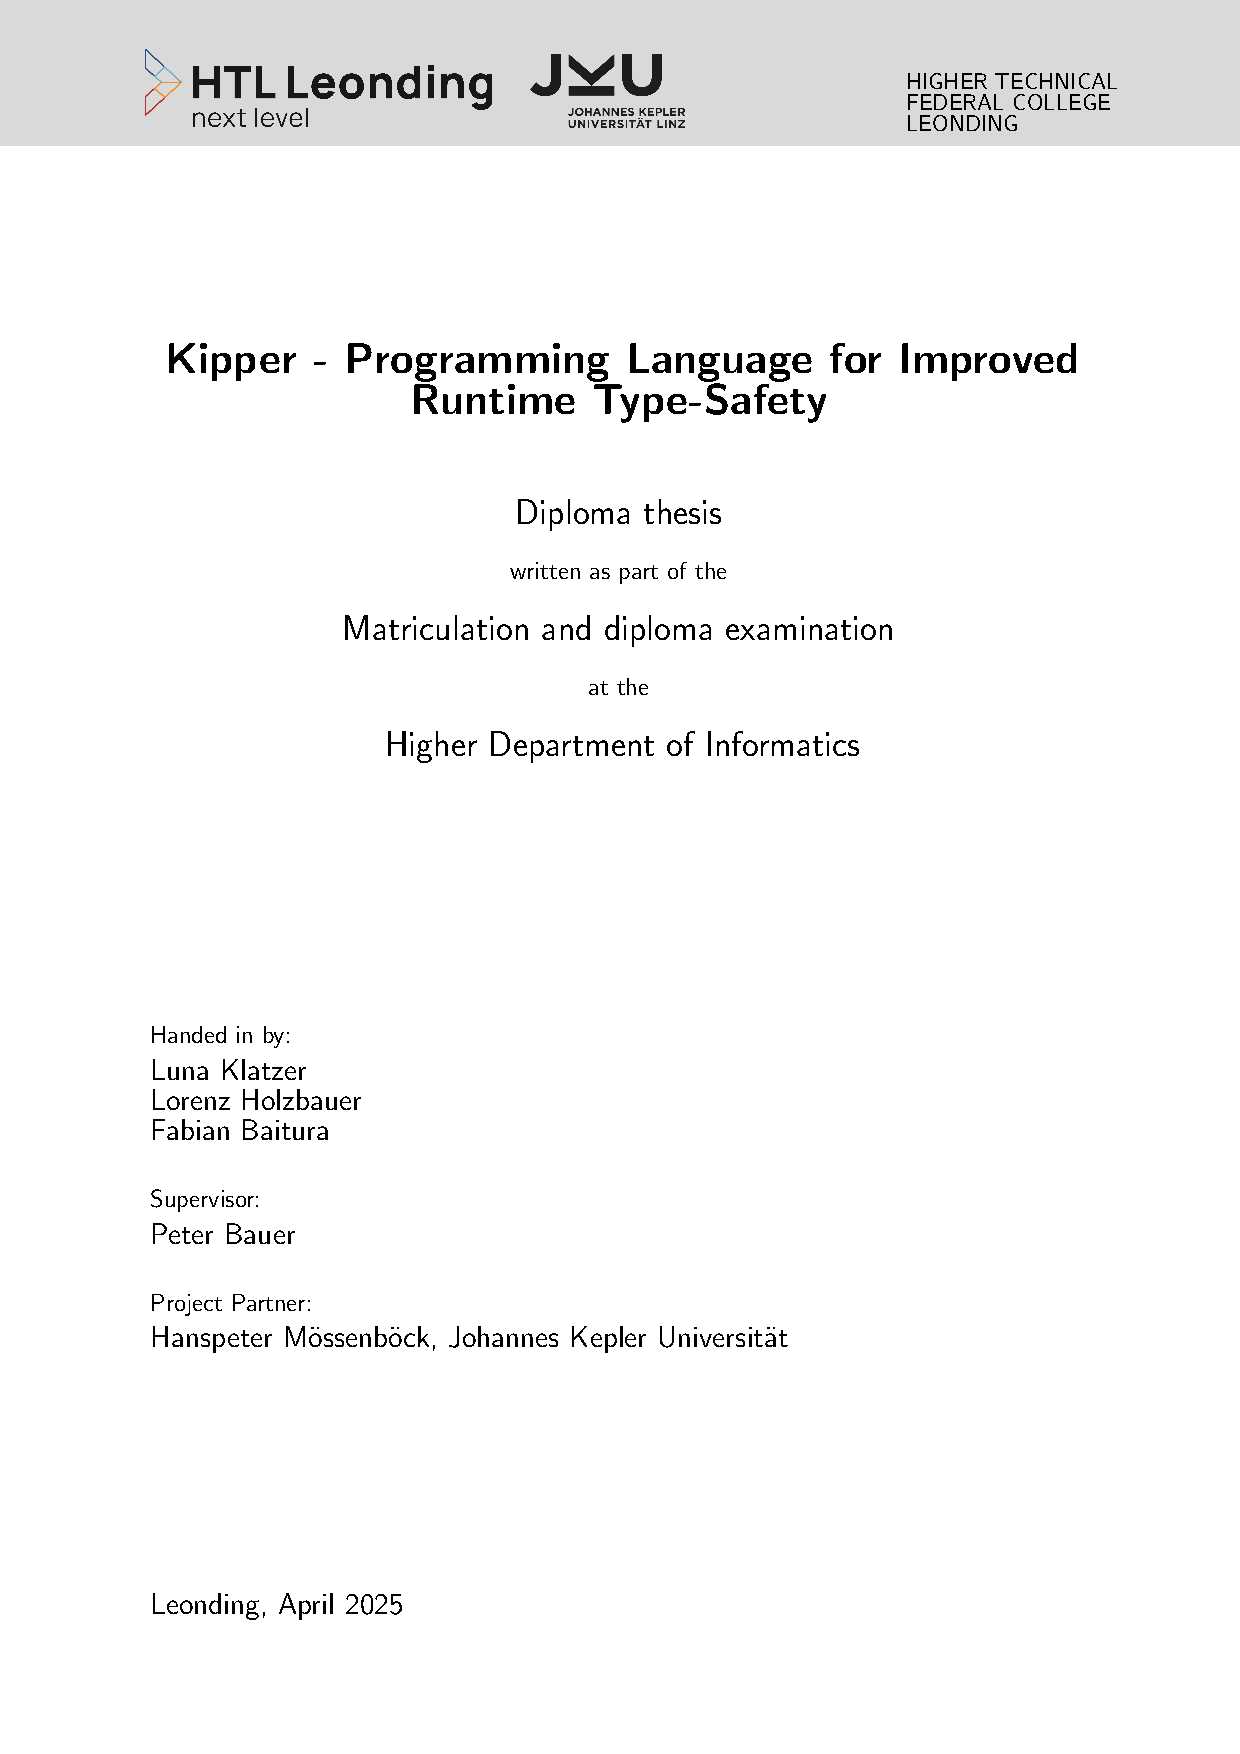
\includepdf{./titlepage/coversheet}
\pagenumbering{Roman}
\newpage
\shipout\null 
\stepcounter{page}
\thispagestyle{empty}
\vspace{3cm}
~ \\ \\
Ich erkläre an Eides statt, dass ich die vorliegende Diplomarbeit selbstständig und ohne fremde Hilfe verfasst, andere als die angegebenen Quellen und Hilfsmittel nicht benutzt bzw. die wörtlich oder sinngemäß entnommenen Stellen als solche kenntlich gemacht habe.

Die Arbeit wurde bisher in gleicher oder ähnlicher Weise keiner anderen Prüfungsbehörde vorgelegt und auch noch nicht veröffentlicht.

Die vorliegende Diplomarbeit ist mit dem elektronisch übermittelten Textdokument identisch.
\vspace{4cm}
% Hier kommt die Unterschrift drüber
\begin{tabbing}
	Leonding, April 2025 \hspace{6.7cm} L. Klatzer \& L. Holzbauer
\end{tabbing}
\vspace{10cm}
\newpage
\setcounter{page}{1}

%%% Local Variables:
%%% mode: LaTeX
%%% TeX-master: "../thesis"
%%% End:
\begin{spacing}{1}
    \chapter*{Abstract}
\end{spacing}
\begin{wrapfigure}{r}{0.4\textwidth}
    \begin{center}
      
\includegraphics[height=0.4\textwidth]{pics/Kipper-Logo.png}
    \end{center}
\end{wrapfigure}

This thesis examines the challenges present in JavaScript environments, particularly the lack of runtime types and comprehensive type safety, and introduces Kipper as a solution. Kipper is a high-level programming language designed to enforce strict type safety at runtime, addressing limitations found in JavaScript and TypeScript, where type correctness is either unchecked or dependent on static analysis tools.

To establish the foundation for Kipper's design, this thesis analyses the JavaScript ecosystem, identifying key issues related to type handling and security. Additionally, potential technologies for implementing Kipper are evaluated, considering their suitability for achieving the project's objectives. Based on this groundwork, the Kipper type system is introduced, incorporating runtime type determination, pattern matching, and interface-based duck typing to enforce type correctness dynamically.

A key focus of this thesis is the development of the Kipper compiler, which translates Kipper code into JavaScript or TypeScript while preserving its type safety mechanisms. The implementation details, including architectural choices and optimizations, are discussed in depth. By addressing the shortcomings of JavaScript and TypeScript, Kipper provides a structured and predictable approach to safer web development. Future work will focus on extending the language's feature set and refining its integration with existing technologies.

\begin{spacing}{1}
	\chapter*{Zusammenfassung}
\end{spacing}
\begin{wrapfigure}{r}{200px}
	\begin{center}
		
\includegraphics[height=200px]{pics/Kipper-Logo.png}
	\end{center}
\end{wrapfigure}

Diese Arbeit untersucht die Herausforderungen in JavaScript-Umgebungen, insbesondere das Fehlen von Laufzeittypen und umfassender Typsicherheit, und stellt Kipper als Lösung vor. Kipper ist eine High-Level-Programmiersprache, die entwickelt wurde, um strenge Typsicherheit zur Laufzeit zu erzwingen. Sie behandelt die Einschränkungen, die in JavaScript und TypeScript zu finden sind, wo die Typkorrektheit entweder ungeprüft oder abhängig von statischen Analysetools ist.

Um die Grundlage für das Design von Kipper zu schaffen, wird in dieser Arbeit das JavaScript-Ökosystem analysiert und die wichtigsten Probleme im Zusammenhang mit der Typbehandlung und Sicherheit identifiziert. Darüber hinaus werden potentielle Technologien für die Implementierung von Kipper auf ihre Eignung zur Erreichung der Projektziele hin untersucht. Auf dieser Grundlage wird das Kipper-Typsystem vorgestellt, das Laufzeit-Typbestimmung, Pattern-Matching und Interface-basiertes Ducktyping zur dynamischen Durchsetzung von Typkorrektheit beinhaltet.

Ein Schwerpunkt dieser Arbeit ist die Entwicklung des Kipper-Compilers, der Kipper-Code in JavaScript oder TypeScript unter Beibehaltung der Typsicherheitsmechanismen übersetzt. Die Implementierungsdetails, einschließlich Architekturentscheidungen und Optimierungen, werden abgewogen. Durch die Behebung der strukturellen Probleme von JavaScript und TypeScript bietet Kipper einen konsistenten und konsequenten Ansatz für eine sicherere Webentwicklung. In der Zukunft wird sich das Projekt auf die Erweiterung des Funktionsumfangs der Sprache und die Verfeinerung der Integration mit bestehenden Technologien konzentrieren.

%%% Local Variables:
%%% mode: LaTeX
%%% TeX-master: "../thesis"
%%% End:

\pagestyle{plain}

\renewcommand{\lstlistlistingname}{List of Source Code Snippets}

\tableofcontents
\newpage
\setcounter{RPages}{\value{page}}
\setcounter{page}{0}
\pagenumbering{arabic}
\pagestyle{scrheadings}

\begin{spacing}{1}
\chapter{Introduction}\label{chapter:introduction}
\end{spacing}
Kipper, formally referred to as the Kipper programming language, is a high-level programming language designed to address various safety issues prevalent in the modern web environment. These issues often arise due to the lack of strict typing and type-checking functionality in JavaScript environments. While some of these issues can be mitigated through the use of linter tools or a compile-time type system, such as the one implemented by TypeScript, they typically rely on the user to correctly identify issues and account for all potential edge cases of an operation. This, however, proves dangerous, as allowing users to manage security within an environment creates a hazard for potential edge cases and complex issues that may not be easily resolved through debugging or detailed program analysis.

Kipper seeks to enhance these existing web languages, such as JavaScript and TypeScript, by offering a runtime environment that includes runtime type checks, type determination, and pattern matching—features previously absent in these ecosystems. This approach allows developers to properly identify types and compare them with defined structures during compile- and runtime, ensuring all aspects of an application are correctly validated. However, Kipper does not aim to replace these languages; rather, it should extend them by providing a comprehensive type system and language that accounts for all edge cases and eliminates untyped or potentially unsafe operations.

To achieve this goal, a compiler was developed as part of this thesis to provide these type safety features while generating output code compatible with both JavaScript and TypeScript environments. It functions similarly to other well-known \gls{transpiler}s, such as the TypeScript transpiler, and operates based on the Kipper programming language. Kipper shares similarities with TypeScript but incorporates syntax elements from other languages, such as Python, to simplify various development processes. Its most significant feature is the Kipper type system, which is inherently strict and definitive, preventing the assignment of incorrect or malformed data. This type system incorporates interface-based duck typing and \gls{object-oriented-programming} (OOP) paradigms to enable flexible yet safe development.

It is important to note that Kipper was not originally conceived as a thesis project or a high-level language in its current form but began as a minor personal project around September 2021. The language evolved over time due to an interest in building upon the JavaScript ecosystem while addressing its commonly perceived limitations. Initially, Kipper incorporated fundamental features such as arithmetic operations, low-level data types, functions, and built-in functions. With the introduction of major features—including error recovery, complex object types, runtime types, and classes—the language has significantly increased in complexity. In its core functionality, Kipper can now be compared to early versions of languages such as JavaScript or Python. This thesis represents a substantial advancement for what was originally a small-scale project. With continued development, Kipper is expected to achieve a full core feature set and direct integration with existing environments in the coming years. However, as of the time of writing, while Kipper is feature-complete within its planned scope, it does not yet include all features commonly found or required in modern programming languages. Essential functionalities such as imports, modules, and asynchronous operations are currently absent from the language.

Furthermore, this thesis should be regarded as a snapshot of the project's development rather than a comprehensive account of its entire history. It primarily focuses on the key features implemented during the 2024/25 period, when Kipper took its current form. Additionally, this thesis does not assert that the language will strictly adhere to all specifications outlined in this paper, nor does it guarantee backward compatibility with the described features. As Kipper remains in active development, it will continue evolving to achieve a standard feature set suitable for a major v1.0 release.

With this in mind, this paper will discuss the background and challenges present in the web environment, examine various aspects of the Kipper compiler—including its design and the decisions made during its development—and inspect the role of Kipper and how it can help achieve a safer development process.

%%% Local Variables:
%%% mode: LaTeX
%%% TeX-master: "../thesis"
%%% End:

\begin{spacing}{1}
\chapter{Background}
\end{spacing}
\section{Dissecting the current issues}
\setauthor{Luna Klatzer \& Lorenz Holzbauer}

\subsection{The JavaScript problem}

Currently, the web space is dominated by JavaScript, a language developed solely for the purpose of creating interactive websites which has become the standard for any modern browser. Originally, when Netscape started development in 1995, it wasn't even intended to get as big as it did, so it comes as no surprise that the programming language, which would become the future of the web, wasn't exactly properly future-proofed or secured for complex operations and architectures.

In the modern age of web development, JavaScript is no longer exclusively a front-end language. Wherever you go you will find JavaScript used in an application. Its usage has grown so much that there is now an incredibly large pool of available frameworks, technologies, and applications that you can use with the language. This though comes with a major problem, since the language powering so many systems today is a fairly harsh environment to work in, as it is filled with many problems ranging from minor inconveniences to major design issues that are impossible to ignore. The most egregious example of this is the type system of JavaScript. It provides neither type checks nor warnings, doesn't allow for objects to be matched against types and requires the user to always know what the value of a variable will be at runtime, making it a constant game of remembering and guessing.

Naturally, as a result, this has caused a lot of solutions to pop up, which all aim to resolve this issue. One of the most well-known and accepted solutions in this regard is TypeScript.

\subsection{TypeScript - One of many solutions}

TypeScript is as of now the most widely used alternative to JavaScript, or more accurately a super-set of it, allowing standard object-oriented functionality and compile-time type-checking similar to that present in Java or C\#. In its core principle, TypeScript provides everything that a developer needs for developing type-safe applications, as you can simply use the type annotations and let the TypeScript compiler check for your errors while working on your project. This though has certain limitations, as TypeScript is bound to the restrictions of a simple linter that aims to be fully compatible with JavaScript, no matter the circumstances. While that allows the developer to import any code from an old code base directly, it also heavily impacts and limits the functionality, which the TypeScript compiler can implement. As a result, the compiler is bound to the constraints of a language that is not even designed for type checking and type annotations. More specifically this means that all type checks are compile-time only and are not checked against at runtime, which means TypeScript works on a trust-based system, where the developer is often used as the root of trust. 

\subsubsection{Unchecked compile-time casts}

As already mentioned TypeScript works on a compile-time-only basis, which does not allow for any runtime type checks. That also naturally means any standard functionality like casts can also not be checked for, since such type functionality requires the language to be able to reflect on its type structure during runtime. Given the fact though that casts, which allow the developer to narrow the type of a value down, are a necessity in everyday programs, TypeScript is forced to provide what you can call "trust-based casts". The developer can, like in any other language, specify what a specific value is expected to be, but unlike usual casts are primarily unchecked, meaning you can, if you want, cast anything to anything with no determined constraint.

While in principle this maintains the status quo and provides the developer with more freedom, it also opens up another challenge that must be looked out for when writing code. If one of those casts goes wrong and isn't actually valid, the developer will only know that at runtime and will have no assistance to fix it. To overcome this developers can themselves implement runtime type checks, which prevent type mismatches in ambiguous contexts. While it is a common approach, it is fairly impractical and adds a heavy burden on the developer as it requires constant maintenance and recurring rewrites to ensure the type checks are up-to-date and valid.

Let's look at an example:

\begin{lstlisting}[language=TypeScript]
class SuperClass {
	name: string = "Super class";
}

class MiddleClass extends SuperClass {
	superField: SuperClass = new SuperClass();
	
	constructor() {
		super();
	}
}

class LowerClass extends MiddleClass {
	classField: MiddleClass = new MiddleClass();
	
	constructor() {
		super();
	}
}

const c1 = <MiddleClass>new SuperClass(); // Unchecked cast
console.log(c1.superField.name); // Runtime Error! Doesn't actually exist

const c2 = <LowerClass>new MiddleClass(); // Unchecked cast
console.log(c2.classField.superField.name); // Runtime Error! Doesn't actually exist
\end{lstlisting}

Here we have a simple example of an inheritance structure, where we access the properties of a child that is itself also another object. Due to the nature of TypeScript operations such as casts are mostly unchecked and usually work on the base of trusting the developer to know what they're doing. That means that in the example given above, the compiler does not realise that the operation the developer is performing is actually invalid and will result in a failure at runtime (can't access property "name", c1.superField is undefined). Furthermore, given that JavaScript only reports on such errors when a property on an undefined value is accessed, the undefined variable may go unused for a while before it is actually the cause of any problem. This leads to volatile code that can in many cases not be guaranteed to work unless the developer actively pays attention to such errors and makes sure that their code does not unintentionally force unchecked casts or other similar untyped operations.

\subsubsection{Ambiguous dynamic data}

Another similar issue occurs when dealing with dynamic or untyped data, which does not report on its structure and as such is handled as if it were a JavaScript value, where all type checks and security measures are disabled. This for one makes sense given the goal of ensuring compatibility with the underlying language, but it also creates another major problem where errors regarding any-typed values can completely go undetected. Consequently, if we were to receive data from a client or server we can not ensure that the data we received is fully valid or corresponds to the expected pattern. This is a problem which neither has a proper workaround nor a solution in TypeScript. 

For example:

\begin{lstlisting}[language=TypeScript]
interface Data {
	x: number;
	y: string;
	z: {
		z1: boolean;
	}
}

function receiveUserReq(): { [key: string]: any } {
	// ...
	return {
		x: "1",
		y: "2",
		z: true
	}
}

var data = <Data>receiveUserReq(); // Unsafe casting with unknown data
console.log(data.z.z1); // No Runtime Error! But returns "undefined"
\end{lstlisting}

For the most part, developers are expected to simply watch out for such cases and implement their own security measures. There are potential libraries which can be utilised to add runtime checks which check the data received, but such solutions require an entirely new layer of abstraction which must be managed manually by a developer. This additional boilerplate code also increases the complexity of a program and has to be actively maintained to keep working. 

Good examples of technologies that provide runtime object schema matching are "Zod" (https://github.com/colinhacks/zod) and "joi" (https://github.com/hapijs/joi). Both are fairly popular and actively used by API developers who need to develop secure endpoints and ensure accurate request data. While they are a good approach to fixing the problem after the fact, they still create their own difficulties. We will examine these later in the implementation section, where we will more thoroughly compare Kipper's approach to other tools.

\section{How could it have been better}

\subsection{Case study: Java}

Java is a statically typed OOP programming language, which is next to C\# one of the primary languages used throughout the world of programming. It runs on a VM-based architecture designed to allow the developer to deploy cross-platform applications and work with powerful dynamic object structures. Like other high-level languages, it provides reflection, a concept essential for the purpose of runtime type checking and validations. Unlike JavaScript or TypeScript, operations in the code are always checked during compile time and runtime if necessary, and can never be simply ignored by the developer. As such when you work with the language and deploy an application you can be sure that the casts and type operations are safe, or at least will have an error thrown in the case of failure. This is a heavy contrast to the entirely dynamic and type-less structure present in JavaScript, which doesn't provide such safeguards and relies on the developer for security. 

\subsection{Case study: Rust}

Rust is a systems programming language designed to offer memory safety without a garbage collector. One of the standout features of Rust is its ownership system, which enforces strict rules for memory allocation and deallocation, preventing common bugs like null pointer dereferencing or data races in concurrent programming. This guarantees memory safety at compile-time without needing a runtime environment to manage memory, unlike languages such as Java and JavaScript, which use garbage collection to manage memory dynamically.

Rust's type system is strongly and statically typed, like Java, but it emphasizes immutability and borrowing concepts to manage data lifetimes and concurrency safely. Unlike Java, Rust does not have reflection, but it provides powerful meta-programming features via macros. Rust also promotes zero-cost abstractions, ensuring that high-level abstractions have no runtime overhead, making it a popular choice for applications requiring both performance and safety. Despite working on the basis of a completely different programming paradigm it still manages to be type-safe or more accurately memory-safe. The compiler makes sure that there are no ambiguities left that could potentially lead to runtime errors and provides absolute safety in a way that still allows certain freedom to the developer.

\subsection{Drawing comparisons to JavaScript}



\section{Tackling the issue at its core}


\begin{spacing}{1}
\chapter{Technology}\label{chapter:tech}
\end{spacing}
\setauthor{Luna Klatzer}

This chapter will discuss the technologies selected and utilized in the Kipper project, detailing their application and comparing them to alternative tools and technologies. It will explore the reasoning behind these choices and evaluate their effectiveness in achieving the project's goals.

\section{Background}
\setauthor{Luna Klatzer}
\label{sec:technology-background}

Before introducing the technologies and tools used in the Kipper project, it is important to note that the project existed on a smaller scale prior to the initiation of this diploma thesis. As such, the following sections will discuss technologies—TypeScript and \Gls{antlr4}—that were chosen before the start of this thesis project. 

Consequently, when the project was re-envisioned and expanded into its current form as part of this diploma thesis, the development technologies had already been determined and were simply continued to build upon the existing foundation.

Nevertheless, to highlight the various alternatives and the reasons behind the original decisions for the parser, lexer, and core compiler, the following sections will still examine each option, assess their viability within the context of this project, and elaborate on the choices made when the initial project was conceived.

\section{Development Language}
\setauthor{Luna Klatzer}
\label{sec:development-language}

The choice of development language, or compiler programming language, is a crucial initial decision when starting a project of this nature. This decision significantly impacts factors such as distribution, accessibility, and cross-platform integration. The selected language sets the foundational conditions for the entire project and influences the ability to effectively utilize the language being created.

Many compilers are initially developed in a different language, often one closely related to the language being designed. Once the language takes on proper shape, the compilers are then often migrated into the newly created language, effectively becoming one of the first test programs to utilize the language directly. This approach allows the compiler to validate its own functionality—serving as a self-serving cycle where each iteration of updates also benefits the compiler itself.

This is not the case here, however. As the Kipper compiler remains too complex for its own language, it is currently written in another language. Nonetheless, the compiler could be migrated to the Kipper language in the future if the required changes are implemented.

\subsection{Selection criteria and weighing the options}
\label{sec:development-language-selection-criteria}

To accurately represent the various benefits and downsides of each individual option, we are going to rank each language based on a set of criteria with individual weights which will amount to a certain total score as presented in Table~\ref{tab:programming-language-criteria-weights}. Based on this score we can accurately represent the viability of each technology option presented.

\begin{table}[H]
	\centering
	\begin{tabular}{ |p{4cm}|p{5cm}|p{5cm}|  }
		\hline
		\multicolumn{3}{|c|}{Weights for the individual criteria} \\
		\hline
		Criterion&Weight between 0.0-1.0&Effective maximum possible score on a scale of 0-100\\
		\hline
		Speed&0.4&40\\
		Maintainability&1.0&100\\
		Platform Support&0.5&50\\
		Extensibility&0.4&40\\
		Similarity to Kipper&0.8&80\\
		\hline
	\end{tabular}
	\caption{Table showcasing the individual criteria for the programming language and their weights}
	\label{tab:programming-language-criteria-weights}
\end{table}

\subsection{Option - C++}
\label{sec:programming-language-option-c++}

C++ is widely recognized as one of the most prominent languages for low-level development and system programming, including compiler development. In addition to offering fast execution speeds, it provides flexible mechanisms like pointers for structuring essential constructs such as trees. The language utilizes OOP (\Gls{object-oriented-programming}) to manage complex structures efficiently and supports templating, often also called generic type parameters, enabling versatile structures with unified behaviour and compatibility.

\subsubsection{Speed}

In terms of speed, C++ is mostly unrivalled, given the output to assembly code that can be directly run on the CPU without any overhead or interpreter. This would allow a compiler to be similarly fast and efficient, allowing even large programs to be compiled and translated quickly.

\subsubsection{Maintainability}

In compiler development, C++ is a common choice due to the wide-spread emphasis on minimizing compilation time and efficient processing of large programs. However, the complexity of memory management and the challenges associated with developing large structures can make C++ difficult to work with, potentially leading to unexpected development issues.

\subsubsection{Platform Support}

Furthermore, targeting multiple environments and systems is challenging, as C++ and by extension C commonly compile directly to machine and os-dependent assembly code, which means compiling the program for each operating system and architecture individually is necessary. Otherwise without virtualisation or subsystems the program can not be executed.

\subsubsection{Extensibility}

Due to the design of C++, the compiled code is largely locked down and any extensions to the compiler would have to be loaded using custom loaders or the user would have to fully re-compile the source code with the wanted changes.

\subsubsection{Similarity to Kipper}

While C++ aims to be more modern compared to its predecessor C, it still is largely a low-level language where programs needs to be structured with a lot of potential edge cases and faults in mind. Kipper on the other hand is a pure high-level \gls{transpilation}-based language with interpreted dynamic targets, so concepts such as memory management, integer sizes and segmentation faults are largely alien. This means if a compiler were to be written in C++, it would require a lot of additional code taking these C++ concepts into account that would have to be removed or heavily altered in a potential succeeding Kipper-based compiler.

\subsection{Option - Java}
\label{sec:programming-language-option-java}

Java is another commonly used OOP language for building compilers and compiler components. As a matter of fact, \Gls{antlr4}, the lexer and parser generation technology, is developed solely in Java and for extended support simply provides output targets for its lexers and parsers used within other languages.

\subsubsection{Speed}

Speed is not a major concern when working with Java. The language and its VM are largely optimised and the JIT (\Gls{just-in-time-compilation}) compiler performs additional optimisations at runtime by analysing the code and the memory of the program. It may in some cases be slower, especially due to the large amount of boilerplate present in a lot of systems, but it can overall be considered fast.

\subsubsection{Maintainability}

Java can be considered a pure OOP programming language, as all executable code is written in class methods, which can be called up and run from other parts of the program. Due to this all functionality adheres to some structure and is usually encapsulated in various classes and methods. While these features alone do not guarantee code that is easy to work with, they simplify that process and provide structures that can be easily changed or altered using inheritance or other functionality. However it often also leads to boilerplate-heavy code that is hard to read especially when programs become complex.

\subsubsection{Platform Support}

Java utilizes a VM in combination with a JIT compiler for executing its intermediate code. This intermediate code is largely system-independent and can be run on any system that has a working Java runtime installed. As such, the responsibility of handling the individual characteristics of each operating system and architecture is left up the Java runtime, which makes compiling fairly simple and allows for a broad support of various systems.

\subsubsection{Extensibility}

Besides providing support for multiple platforms, the architecture of Java allows it to be an easy language to set up and extend, as its modularity means loading additional code simply means compiling it to the same standardised intermediate format. Using a class loader, this new runnable code can be then picked up at runtime and immediately executed. Additionally, the source code classes can be referenced and used within subsequent implementations that extend the original compiler functionality.

\subsubsection{Similarity to Kipper}

Java is fairly similar to Kipper in its OOP design paradigm, but is still generally very different. Kipper runs as JavaScript or TypeScript in an interpreted environment, where code is ran line per line. While this is similar to the JIT compiler utilised by Java, Kipper can run high-level code and execute on-demand changes without compiling its code or having to generate intermediate code. Given though that structurally the two languages are very similar, migrating from a compiler written in Java to one written in Kipper would be mostly straightforward.

\subsection{Option - TypeScript}
\label{sec:programming-language-option-typescript}

TypeScript is a super-set of JavaScript, which works on the same dynamically-typed and interpreted system and is during runtime de-facto the same language. As such, it is generally not preferred when it comes to implementing a compiler, since its dynamic structure and functionality do not serve a lot of use in a compiler with very specific functionality and limit performance. Still, it is often used for experiments and online compilers, which may not perform as well, but can still achieve good performance.

\subsubsection{Speed}

In terms of speed, TypeScript can be very fast, almost as fast as WASM (\Gls{webassembly}) in some cases. Although it still generally has the same limitations as any other web language. Given that the language needs interpretation and does not utilise JIT compilation or a compiled format, it often can not compete with languages such as Java, C++ or C\#. Still, with its heavily optimised interpreter regular algorithms and programs can be fast, but as complexity grows it is not as efficient as comparable languages.

\subsubsection{Maintainability}

In terms of maintainability TypeScript is generally regarded as maintainable, due to its simplified interpreter structure and detailed compiler errors, but also as problematic due to its common problems that are caused by its own compile-time only types and limitations in performing proper runtime checks or accounting runtime values into a given program. Great care must be put how specific operations are performed and how dynamic data is handled, as errors can easily occur due to oversight or negligence in appropriate type checks.

\subsubsection{Platform Support}

TypeScript, or its generated JavaScript counterpart, can run on any system that has a browser or a local browser-like counterpart like \Gls{nodejs}, \Gls{deno} or \Gls{bun} installed. However, every version of the JavaScript interpreprogramming-language-criteria-weightster comes with its own limitations and even in browsers running code can cause problems across various systems. This is more noticeable with locally installed systems such as \Gls{nodejs}, \Gls{deno} or \Gls{bun}, which implement their own libraries and design systems that need to be accounted for. Generally it can be said though that if the correct environment is set up, the code can run on any OS or architecture without issue. In the case of a standard browser, this often becomes even more simple, as browsers try to largely implement the same standards and concepts so that websites and their JavaScript code can run with identical results.

\subsubsection{Extensibility}

TypeScript is a very dynamic language with a lot of flexibility in terms of extending and modifying structures with ease. Even if a compiler were not able to support modifications, hooking into the object and modifying it if needed is relatively easy. Additionally by simply providing interfaces and specific arguments that need to be implemented a compiler could allow custom classes and data to be executed. Furthermore, referencing the original classes and objects is fairly simple and like Java can be used for subsequent implementations and custom versions of the compiler.

\subsubsection{Similarity to Kipper}

TypeScript serves as the primary inspiration for Kipper and shares many similarities with it, despite its limitations and challenges related to type safety. This similarity arises from Kipper's design goal of maintaining compatibility with the JavaScript ecosystem and extending it in a type-safe manner. Consequently, Kipper avoids incorporating functionality or design structures that could break compatibility with existing JavaScript tools and frameworks. With this in mind, theoretically any TypeScript code could be inserted into Kipper with only certain syntax changes and type safety changes necessary.

\subsection{Result}

Based on the analysis performed on each of the options listed in sections~\ref{sec:programming-language-option-c++},~\ref{sec:programming-language-option-java} and~\ref{sec:programming-language-option-typescript}, the following results were determined as presented in Table~\ref{tab:programming-language-results}.

\begin{table}[H]
	\centering
	\begin{tabular}{ |p{2cm}|p{1.8cm}|p{1.8cm}|p{1.8cm}|p{1.8cm}|p{1.8cm}|p{1.2cm}|  }
		\hline
		\multicolumn{7}{|c|}{Result values for the criteria selected in~\ref{sec:development-language-selection-criteria}} \\
		\hline
		Language&Speed&Maintain- ability&Platform Support&Extensi- bility&Similarity to Kipper&Result\\
		\hline
		C++&40&50&20&10&30&150\\
		Java&35&80&40&30&55&240\\
		TypeScript&25&70&50&40&70&255\\
		\hline
	\end{tabular}
	\caption{Table showcasing the individual criteria and the scores each language scored}
	\label{tab:programming-language-results}
\end{table}

As presented in the Table~\ref{tab:programming-language-results}, C++ is the least adequate with 150 points scored, Java is largely satisfactory in second place with its 240 points scored and TypeScript is the most suitable with 255 points in total. While TypeScript did not score as well as the other two in the "Speed" criterion, it was mostly first place or close behind Java in all other criteria.

This result supports the pre-existing decision presented in Section~\ref{sec:technology-background}.

\section{Parser \& Lexer Technology}
\setauthor{Luna Klatzer}

The choice of parser and lexer technology, alongside the development language, is a critical factor in the efficiency, extensibility, and maintainability of a programming language. Parsing is inherently complex and can contribute significantly to compilation time. While many language compilers implement custom parsers from scratch to optimise efficiency and minimise execution time, employing parser and lexer generation technology can offer notable advantages.

Using a parser and lexer generator provides greater flexibility, allowing modifications to the language grammar with minimal effort. Additionally, these tools often support multiple languages and compilation targets, enhancing adaptability if the language evolves or expands to additional platforms in the future.

\subsection{Selection criteria and weighing the options}
\label{sec:parser-and-lexer-technology-selection-criteria}

To accurately represent the various benefits and downsides of each individual option, we are going to rank each technology based on a set of criteria with individual weights which will amount to a certain total score as presented in Table~\ref{tab:parser-and-lexer-technology-selection-criteria}. Based on this score we can accurately represent the viability of each parser \& lexer generator option presented.

\begin{table}[H]
	\centering
	\begin{tabular}{ |p{4cm}|p{5cm}|p{5cm}|  }
		\hline
		\multicolumn{3}{|c|}{Weights for the individual criteria} \\
		\hline
		Criterion&Weight between 0.0-1.0&Effective maximum possible score on a scale of 0-100\\
		\hline
		Speed&0.6&60\\
		Integration&1&100\\
		Maintainability&0.8&80\\
		\hline
	\end{tabular}
	\caption{Table showcasing the individual criteria for the parser \& lexer technology and their weights}
	\label{tab:parser-and-lexer-technology-selection-criteria}
\end{table}

\subsection{Option - Antlr4}
\label{sec:parser-technology-option-antlr4}

\Gls{antlr4} is one of the most widely used lexer and parser generators employing a top-down LL(*) parsing process, offering a comprehensive set of tools and multiple output targets, including a target for native TypeScript. It processes Antlr-specific grammar files and, based on the defined tokens and syntax rules, generates both a lexer and a parser, which are individually executable. Using either a listener or a visitor approach, the resulting parse tree can be traversed and transformed into an AST (\Gls{abstract-syntax-tree}) for subsequent compilation~\cite{antlr}.

Although \Gls{antlr4} provides extensive tooling and allows for the extraction of detailed metadata from source code, its generated lexer and parser are generally not considered highly performant compared to the alternatives. Parsing can take a significant amount of time, particularly for large programs. While \Gls{antlr4} employs various optimisation techniques—such as improving performance over time as the parser "warms up" and refines its internal connections—the generic design and modularity introduce overhead that hinders performance optimisations commonly found in other parsing technologies.

Additionally, \Gls{antlr4} generates detailed objects and multiple context objects for each token and tree node, leading to high memory consumption. However, in most modern use cases, this is not a major concern.

\subsection{Option - Coco/R}
\label{sec:parser-technology-option-coco}

Coco/R is a compiler generator that, based on a grammar file, produces a scanner (lexer) and parser employing top-down LL(*) parsing capable of validating the syntactic integrity of a file while also performing semantic and type analysis. Unlike a pure lexer and parser generator, Coco/R integrates aspects of semantic analysis into its processing, thereby optimising performance by preemptively conducting checks that do not require complex context-based analysis~\cite{coco}~\cite{coco-manual}.

By instantiating the scanner and parser within a compiler class, Coco/R-generated classes can be used in a manner similar to \Gls{antlr4}. However, for generating an AST, Coco/R grammars can be directly configured to construct a tree and build individual custom nodes, similar to the process of generating a parse tree. Using the generated AST, subsequent processing and translation can be performed in a manner nearly identical to \Gls{antlr4}~\cite{coco-ast}.

Unlike \Gls{antlr4}, however, Coco/R does not provide an explicit target for TypeScript. Supporting TypeScript would require either implementing a custom target or translating the generated C\# or Java code into WASM, which could then be executed within a TypeScript context. Both approaches would require significant development effort but could likely surpass \Gls{antlr4} in performance.

\subsection{Option - GNU Bison}
\label{sec:parser-technology-option-bison}

GNU Bison is a parser generator that employs a bottom-up LR parsing algorithm to validate the syntactic structure of an input token stream~\cite{bison}. Unlike \Gls{antlr4} or Coco/R, Bison primarily generates parsers for C and C++, with an experimental Java target also available. This focus on lower-level languages provides performance advantages, as Bison is highly efficient~\cite{bison-manual}.

Bison processes a grammar definition file and generates a parser that integrates with a lexer, typically implemented using Flex~\cite{flex}. While it offers strong performance, it lacks a native TypeScript target. Integrating Bison with a TypeScript-based project would require running the generated C/C++ code via WASM like in the case of Coco/R, adding complexity and overhead due to the additional process layer. Important to also mention is that its tooling and extensibility are less modern compared to \Gls{antlr4} and the tool is heavily based on traditional compilers.

Despite these challenges, Bison is a good choice for performance-critical applications where an LR parser is preferred and cross-language execution is acceptable.

\subsection{Option - Custom Implementation}
\label{sec:parser-technology-option-custom}

A custom implementation provides full control over the lexer, parser, and subsequent processing, making it a suitable option for projects with specific requirements or performance constraints. By manually designing a lexer and parser in TypeScript, both speed and memory usage can be optimised while avoiding the overhead associated with general-purpose parser generators.

The primary advantage of a custom parser is its flexibility. Unlike for example \Gls{antlr4} or Bison, it can be precisely tailored to the needs of the project, reducing unnecessary complexity. However, this approach demands significant development effort, including manual error handling and debugging, which can be complex and time-consuming.

Additionally, developing a lexer and parser requires a deep understanding of parsing algorithms and careful handling to prevent ambiguity errors and incorrect results. In many cases, a custom implementation may ultimately be slower and less flexible than using a parser generator, as the latter benefits from years of optimisation and widespread use in compiler design, which is hard to compete with without extensive knowledge.

\subsection{Result}

Based on the analysis performed on each of the options listed in sections~\ref{sec:parser-technology-option-antlr4},~\ref{sec:parser-technology-option-coco},~\ref{sec:parser-technology-option-bison} and~\ref{sec:parser-technology-option-custom}, the following results were determined as presented in Table~\ref{tab:parser-and-lexer-technology-results}.

\begin{table}[H]
	\centering
	\begin{tabular}{ |p{3.2cm}|p{2.8cm}|p{2.8cm}|p{2.8cm}|p{1.6cm}|  }
		\hline
		\multicolumn{5}{|c|}{Result values for the criteria selected in~\ref{sec:parser-and-lexer-technology-selection-criteria}} \\
		\hline
		Technology&Speed&Integration&Maintainability&Result\\
		\hline
		Antlr4&35&90&70&195\\
		Coco/R&50&40&50&140\\
		GNU Bison&50&40&40&130\\
		Custom&25&100&20&145\\
		\hline
	\end{tabular}
	\caption{Table showcasing the individual criteria and the scores each technology scored}
	\label{tab:parser-and-lexer-technology-results}
\end{table}

As presented in Table~\ref{tab:parser-and-lexer-technology-results}, Bison is the least suitable option, scoring 130 points, followed by Coco/R with 140 points. A custom implementation ranks second-best with 145 points, while \Gls{antlr4} emerges as the most suitable choice with 195 points.

Despite their performance and capabilities, both Coco/R and Bison present significant drawbacks, primarily due to their poor integration within the target environment and the additional development effort required for full utilisation. 

Furthermore, while a custom parser implementation offers advantages in flexibility and control, it would likely under-perform compared to other options and demand substantial effort to maintain and develop further.

This result supports the pre-existing decision presented in Section~\ref{sec:technology-background}.

%%% Local Variables:
%%% mode: LaTeX
%%% TeX-master: "../thesis"
%%% End:

\begin{spacing}{1}
\chapter{Implementation}\label{chapter:implementation}
\end{spacing}
\section{Compiler}
\label{sec:compiler}
\setauthor{Luna Klatzer}

The Kipper Compiler is the core component of the Kipper project, serving as the central piece connecting the Kipper language to its target environment. It functions similarly to other \gls{transpilation}-based compilers, such as the TypeScript compiler, by producing high-level output code from high-level input code—specifically, code written in the Kipper language. The syntax of the language is predefined and implemented using the lexer and parser generated by the \Gls{antlr4} parser generator. 

An interesting aspect of the Kipper compiler is its largely modular design, which allows various components to be replaced or extended as needed. This modularity primarily serves to enable the compiler's structure to adapt to future changes in the language and its target output environment. Given the rapid evolution of web technologies and the frequent addition of new functionality, it is essential to ensure that the compiler remains current. Additionally, this design allows users to create plugins or extensions for the compiler to support custom functionality that may not be natively available.

Furthermore, as discussed in greater detail in section~\ref{sec:output-generation}, the compiler is capable of targeting more than one output format. Specifically, it supports both standard JavaScript, adhering to the ES6/ES2015 specification, and standard TypeScript as defined by Microsoft. Similar to other compiler systems, users can configure the compiler according to their preferences and specify the desired target language.

\subsection{Stages of compilation}
\setauthor{Luna Klatzer}

The Kipper compiler processes the program through multiple phases, each building upon the previous one to progressively enrich the semantic and logical representation of the program. The phases and their corresponding responsible components are as follows:

\subsubsection{Lexical Analysis}
\begin{itemize}
	\item Detailed explanation in section~\ref{sec:lexing-parsing}
	\item Performed by: Antlr4 Kipper Lexer
	\item This phase tokenizes the source code into a stream of lexemes, identifying the basic units of syntax.
\end{itemize}

\subsubsection{Syntax Analysis - Parsing}
\begin{itemize}
	\item Detailed explanation in section~\ref{sec:lexing-parsing}
	\item Performed by: Antlr4 Kipper Parser
	\item In this phase, the lexed tokens are organized into a parse tree based on the grammar rules of the Kipper language.
\end{itemize}

\subsubsection{Parse Tree Translation to AST}
\begin{itemize}
	\item Detailed explanation in section~\ref{sec:translation-to-the-ast}
	\item Performed by: Kipper Core Compiler
	\item Converts the parse tree into an Abstract Syntax Tree (AST), a more abstract and language-independent representation of the code.
\end{itemize}

\subsubsection{Semantic Analysis}
\begin{itemize}
	\item Detailed explanation in section~\ref{sec:semantic-analysis}
	\item Performed by: Kipper Core Compiler
	\item This phase is split into three separate steps:
	\begin{enumerate}
		\item Primary Semantic Analysis: Validates language semantics such as variable declarations and scope resolution.
		\item Preliminary Type Analysis: This phase performs initial type validations and checks. It includes tasks such as loading type definitions that might be referenced elsewhere in the program. These types need to be pre-loaded to ensure they are available and correctly resolved during subsequent stages of compilation.
		\item Primary Type Analysis: Conducts in-depth type validation and resolves type-related issues for the given statements and expressions.
	\end{enumerate}
\end{itemize}

\subsubsection{Target-Specific Requirement Checking}
\begin{itemize}
	\item Detailed explanation in section~\ref{sec:translation-to-the-ast}
	\item Performed by: Target Semantic Analyser
	\item Ensures compliance with the specific requirements of the target platform (JavaScript or TypeScript).
\end{itemize}

\subsubsection{Optimization}
\begin{itemize}
	\item Detailed explanation in section~\ref{sec:translation-to-the-ast}
	\item Performed by: Kipper Core Compiler
	\item Performs code optimizations, currently focused on treeshaking to eliminate unused code.
\end{itemize}

\subsubsection{Target-Specific Translation}
\begin{itemize}
\item Detailed explanation in section~\ref{sec:output-generation}
\item Performed by: Target Translator
\item Translates the optimized AST into the desired target language (JavaScript or TypeScript).
\end{itemize}

Each phase of the compiler is executed sequentially, with each step requiring the successful completion of the previous one. This ensures that each module of the compiler can safely rely on the correctness and completeness of the information provided by earlier steps. However, this approach limits the compiler's ability to recover from errors or detect all faults in a single execution. As a trade-off, this method simplifies the implementation and reduces overall complexity. Unlike TypeScript, for example, this means that the compiler cannot ignore certain errors and work around them. 

\section{Lexing \& Parsing}
\label{sec:lexing-parsing}
\setauthor{Luna Klatzer}

The first step in the compilation process is the lexing and parsing of the input program. This involves the tokenization of the program source code, where individual strings are classified into predefined categories, followed by syntactical analysis that organizes these tokens into statements, expressions, and declarations.

In the Kipper compiler, these two steps are carried out by the Kipper Lexer and Parser generated by \Gls{antlr4}, rather than being directly implemented within the compiler itself. These \Gls{antlr4}-generated components are constructed based on the predefined token and syntax rules specific to the Kipper language.

\subsection{Syntax definition}

The primary utility provided by \Gls{antlr4} lies in its ability to generate lexers and parsers automatically from an input file written in the Antlr4-specific ".g4" context-free grammar format. For Kipper, the lexer and parser each have distinct definitions, specifying the individual tokens and the rules for constructing the syntax tree that organizes and groups these tokens.

These definitions are created in a manner similar to other syntactical specification methods, such as \acrshort{bnf} (Backus-Naur Form), commonly used for context-free formal grammars. However, unlike \acrshort{bnf}, Antlr4 grammars have the added capability to include programmatic conditions and invocations, enabling more dynamic and adaptable grammar definitions.

\subsubsection{Lexer Grammar Definition}
\label{sec:lexer-grammar-definition}

In the case of the Kipper Lexer, it uses its own token definition file, which defines how characters are grouped into tokens. This file specifies the rules for identifying individual tokens while ignoring special characters that are not required for syntax analysis. Additionally, the lexer separates the matched tokens into various channels, allowing for more efficient handling and categorization during subsequent parsing steps. (see~\ref{sec:token-channels} for more detail)

For example, in Kipper, the lexer grammar includes constructs for identifying both comments and language-specific keywords. These definitions can be seen showcased below in listing~\ref{lst:kipper-lexer}.

\begin{lstlisting}[language=antlr4, caption={Sample snippet from Kipper Lexer grammar}, label={lst:kipper-lexer}]
	BlockComment : '/' .? '*/' -> channel(COMMENT) ;
	
	LineComment : '//' CommentContent -> channel(COMMENT) ;
	
	Pragma : '#pragma' CommentContent -> channel(PRAGMA) ;
	
	InstanceOf : 'instanceof';
	
	Const : 'const';
	
	Var : 'var';
\end{lstlisting}

In the grammar above, comments are directed to a separate channel using the \lstinline|-> channel| annotation. This helps isolate them from the main parsing flow while still retaining them for potential processing or documentation purposes. Pragmas, which are typically compiler directives, are handled similarly but redirected to a \lstinline|PRAGMA| channel.

\Gls{antlr4} grammars also include support for defining keywords, operators, and contextual language constructs. For instance, \lstinline|Const| and \lstinline|Var| are tokenized as reserved keywords, ensuring they are recognized unambiguously during lexical analysis. This explicit tokenization is critical for constructing a clear and predictable syntax tree, which serves as the foundation for the subsequent phases of interpretation and compilation.

\subsubsection{Syntactical Grammar Definition}
\label{sec:parser-grammar-definition}

Like the Kipper Lexer, the Kipper Parser is defined by its own syntax definition file. In this file, various rules are grouped into syntax rules that collectively form a hierarchical structure. The parser traverses this structure to determine which syntactical construct is represented by the individual tokens. These syntax rules are organized in a way that allows the parser to construct a parse tree by following specific paths, with each path representing a distinct syntactical structure in the Kipper language.

For example, a grammar rule defining a function declaration in Kipper could be expressed as seen in listing~\ref{lst:function-declaration}:

\begin{lstlisting}[language=antlr4, caption={Function Declaration Grammar}, label={lst:function-declaration}]
	functionDeclaration : 'def' declarator '(' parameterList? ')' '->' typeSpecifierExpression compoundStatement? ;
	
	parameterList : parameterDeclaration (',' parameterDeclaration)* ;
	
	parameterDeclaration : declarator ':' typeSpecifierExpression ;
\end{lstlisting}

In this grammar, the rule for \lstinline|functionDeclaration| begins with the keyword \lstinline|'def'|, followed by a \lstinline|declarator| (which represents the function name or identifier), and then an optional \lstinline|parameterList|. The rule includes a \lstinline|typeSpecifierExpression|, indicating the return type of the function, and optionally a \lstinline|compoundStatement|, which represents the function's body.

The \lstinline|parameterList| rule handles the optional inclusion of one or more parameters, each defined by \lstinline|parameterDeclaration|. Each \lstinline|parameterDeclaration| consists of a \lstinline|declarator| (the parameter's name) followed by a type specification. This structure clearly defines the expected syntax for a function declaration in Kipper, ensuring that the parser can accurately identify and process this construct.

Using these syntax rules, the Kipper parser can build a detailed parse tree, with nodes representing various language constructs, such as function definitions, parameters, and expressions. This hierarchical structure allows for efficient interpretation or compilation of Kipper code.

\subsection{Lexical analysis}

\subsubsection{Primary tokenisation}

The primary task of the lexical analysis is the tokenisation of the individual characters into grouped tokens which represent syntactical elements, such as identifiers, keywords, constant values, etc. Tokens serve as the building blocks for higher-level constructs in the parsing process, providing a simplified and structured representation of the raw source code.

The step of tokenisation is fairly straightforward as it simply follows the definitions provided in the grammar file (see~\ref{sec:lexer-grammar-definition}) and throws errors in case no associated token definition is found. Each token is assigned a specific type based on the grammar rules, ensuring that the source code adheres to the language's syntactical structure. If a character sequence does not match any defined rule, an error is raised, indicating the presence of invalid syntax.

The lexer operates as a state machine, scanning through the input character stream and categorizing sequences based on patterns defined in the grammar. These patterns may include regular expressions to match identifiers, numerical constants, or specific language keywords. Once tokens are identified they are put into the associated channels as explained in~\ref{sec:token-channels}.

\begin{figure}[h!]
	\centering
	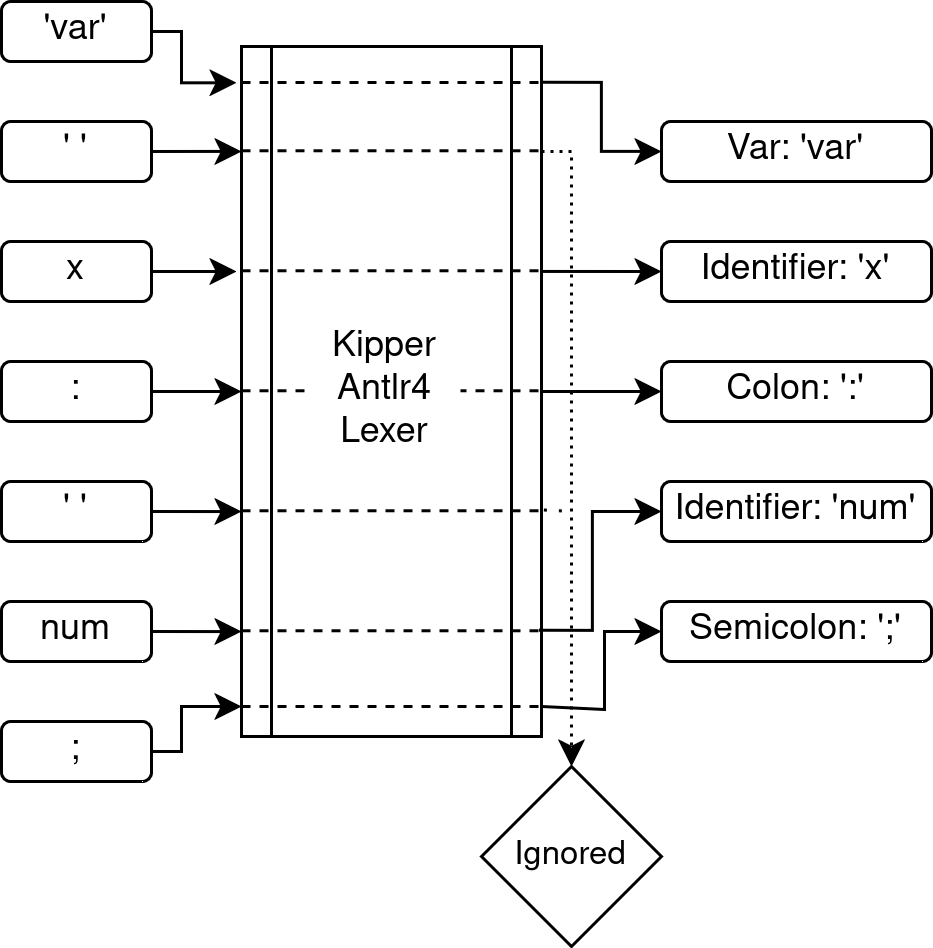
\includegraphics[scale=1]{./pics/Lexer-Algorithm.drawio}
	\caption{The lexing process which categories the various tokens}
	\label{fig:implementation:Lexer-Algorithm}
\end{figure}

\subsubsection{Token Channels}
\label{sec:token-channels}

Next to the definition of the various tokens the grammar file also specifies what channel each token should be put into. These channels act as a stream of tokens where each stream represents different semantic parts of the program.

The channels which are implemented in the case of Kipper are:

\begin{itemize}
	\item \textbf{Default channel}
	\item \textbf{Comments channel}
	\item \textbf{Pragma channel}
	\item \textbf{Ignored channel}
\end{itemize}

The \textbf{default channel} serves as the primary stream, storing nearly all tokens in the program. It is the main channel used during the parsing step to construct a parse tree of the program.

The remaining channels are special-purpose streams that are excluded during parsing and cater to specific functionalities:

\begin{itemize}
	\item The \textbf{comments channel} is dedicated to storing all comments, which are logically irrelevant to the program and do not require parsing or further processing.
	\item The \textbf{pragma channel} contains compiler pragmas—special instructions to the compiler that are processed independently from the standard syntax rules.
	\item The \textbf{ignored channel} is reserved for special characters that are significant only for token differentiation but have no logical relevance to the program, such as spaces. While spaces are critical for separating tokens, like with \lstinline|var x| and \lstinline|varx| they do not contribute to the program's logic and are therefore excluded from parsing.
\end{itemize}
	
\subsubsection{Nested Sub-Lexing}
\label{sec:nested-sub-lexing}

Besides standard sequential processing of the input, the Kipper Lexer also employs a technique called sub-lexing. Sub-lexing involves branching off the main lexing process and invoking a sub-lexer that operates under its own set of rules and guidelines. This specialized lexer handles specific subsets of tokens that require unique processing rules.

Sub-lexing is crucial for Kipper due to features such as templating, where code fragments are embedded within strings. In such cases, the lexer must correctly differentiate between string elements and code atoms (the inserted snippets inside the string). By using a simple push-and-pop mechanism, the lexers can function similarly to a stack, layering processing contexts on top of one another. Each context processes its corresponding string subset, enabling correct parsing of both regular syntax and embedded code within strings. This modular approach ensures cleaner handling of complex tokenisation scenarios and increases the lexer's flexibility.

\begin{figure}[h!]
	\centering
	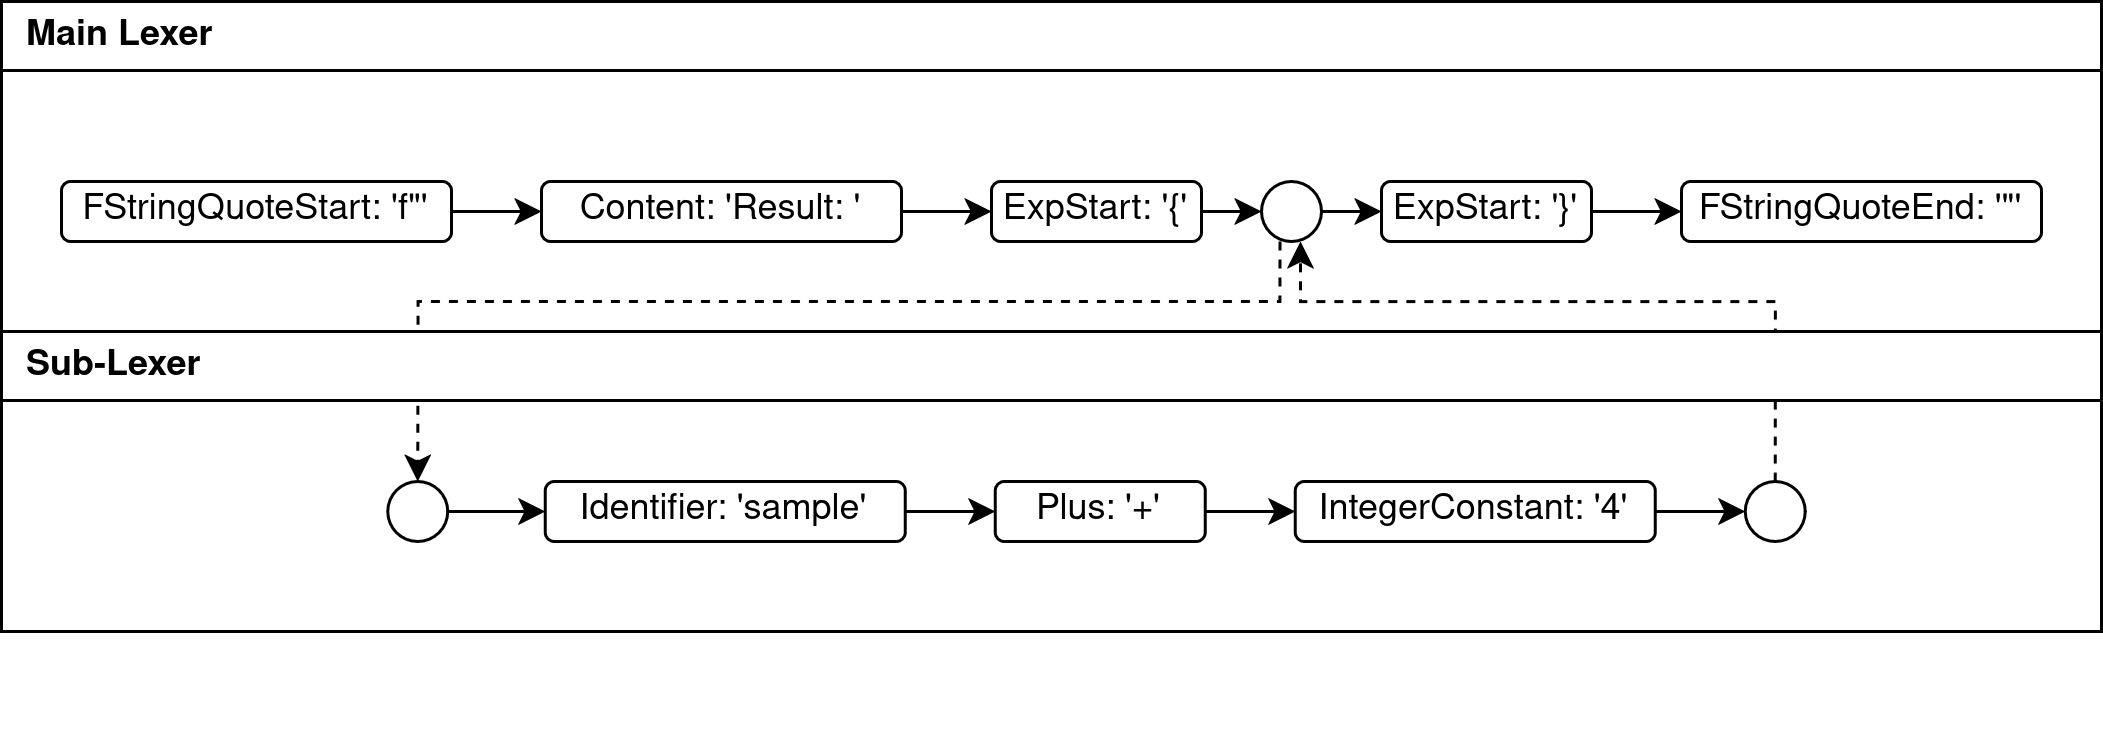
\includegraphics[scale=0.85]{./pics/Sub-Lexer.drawio}
	\caption{The process of invoking a sub-lexer with the sample input \lstinline|f"Result: \{sample + 4\}"| (An example of a template string, or also format string, in the Kipper language), where all content between \lstinline|\{| and \lstinline|\}| is passed onto the sub-lexer.}
	\label{fig:implementation:sub-lexer}
\end{figure}

\subsection{Syntactic analysis}

\subsubsection{Primary syntactic analysis of the token stream}

With the lexer having already identified all tokens in a given program and ensured that only valid elements are present, the parser proceeds to analyse the program's structure and logic. This step is inherently more complex and often demands a significant amount of processing time. The complexity arises partly from the computational effort required to transform a token stream into a viable syntax tree and partly from the design of \Gls{antlr4}, which generates detailed context objects for each node in a program and as such requires a lot of memory and processing to call up each context.

The parser's primary task is to verify that the sequence of tokens conforms to the grammatical rules specified by the Kipper grammar. This involves checking whether constructs such as statements, expressions, and control structures are correctly formed.

\subsubsection{Building the parse tree}

Similar to the hierarchical structure defined by Kipper's grammar rules, the parse tree generated by the Kipper Parser also exhibits a hierarchical organization. Each parse node may have multiple child nodes and is connected to a single parent node, positioned syntactically one level higher within the tree. These nodes can either represent a rule node, such as \lstinline|expression|, or correspond directly to a simple lexer token.

The construction of a parse tree begins with a designated root node representing an entire file. From this root, branching occurs through intermediate rule nodes that capture various grammatical constructs, such as statements, definitions and expressions. These intermediate nodes eventually lead to leaf nodes, which are simple lexer tokens forming the smallest syntactic components of the program, such as identifiers, keywords, operators, and literals.

This hierarchical structure enables easy traversal and analysis of the program during later stages of compilation or interpretation. For instance, an arithmetic expression in a program, such as \lstinline|a + b * c|, would form a sub-tree where the root node corresponds to an expression rule, with child nodes representing the individual terms and operations in the correct precedence order.

A simplified representation of this tree structure is shown in figure~\ref{fig:implementation:parse-tree}.

\begin{figure}[h!]
	\centering
	\includegraphics[scale=0.95]{./pics/Parse-Tree.drawio}
	\caption{A simplified parse tree representation of the statement \lstinline|var x: num = 4;|.}
	\label{fig:implementation:parse-tree}
\end{figure}

\subsubsection{Programmatic conditions \& context-sensitive rules}

In addition to standard context-free rules, there are grammar rules that incorporate programmatic conditions, requiring specific requirements to be met beyond the standard syntactic structure. These rules are inherently context-sensitive, as they cannot be identified without considering the program’s position and overall logic.

An example of a context-sensitive rule is the compound statement \lstinline|{ }|, which groups multiple statements and is typically used as the body of functions and methods. By definition, such statements are generally permitted only as top-level program nodes or as children of other statements, excluding cases where expressions such as lambda expressions specify one as a child. To accommodate lambdas having a structured body, two types of compound statements are defined. While they serve the same practical purpose, they are logically different due to their different contexts of usage: one as a child of another statement and another as a child of a lambda expression.

\subsection{AST (Abstract Syntax Tree)}
\label{sec:translation-to-the-ast}

The \acrshort{ast} represents a tree which groups together the most logically essential elements of a specific items and disregards all the other items not necessary in further processing. Lexer tokens, such as \lstinline|:|, \lstinline|=| or \lstinline|;| may be important syntactically as indicators for specific operations and structures, but once a specific parser rule kind has been determined and the meaning can be derived from that alone these tokens are not necessary anymore and can be discarded.

\subsubsection{Parse Tree Walking}

To transform the parse tree generated by the Kipper Parser, the compiler uses a tree-walking algorithm that systematically traverses the tree by entering and exiting grammar rules. During this process, the algorithm invokes specific handlers when they are defined for particular parse nodes. These handlers are designed to process only the most significant parse nodes, which typically correspond to essential syntactic constructs of the source code.

When a handler is called, it constructs a new \acrshort{ast} node and attaches it to the growing \acrshort{ast}. This selective processing approach ensures that irrelevant parse tree details, such as redundant intermediate nodes or syntactic artifacts, are automatically excluded from the \acrshort{ast}. The resulting \acrshort{ast} is a simplified and more abstract representation of the program's structure, capturing only the semantically relevant elements needed for subsequent stages of the compilation process.

The \acrshort{ast} generation result of such a tree walk process can be seen in figure~\ref{fig:implementation:ast}.

\begin{figure}[h!]
	\centering
	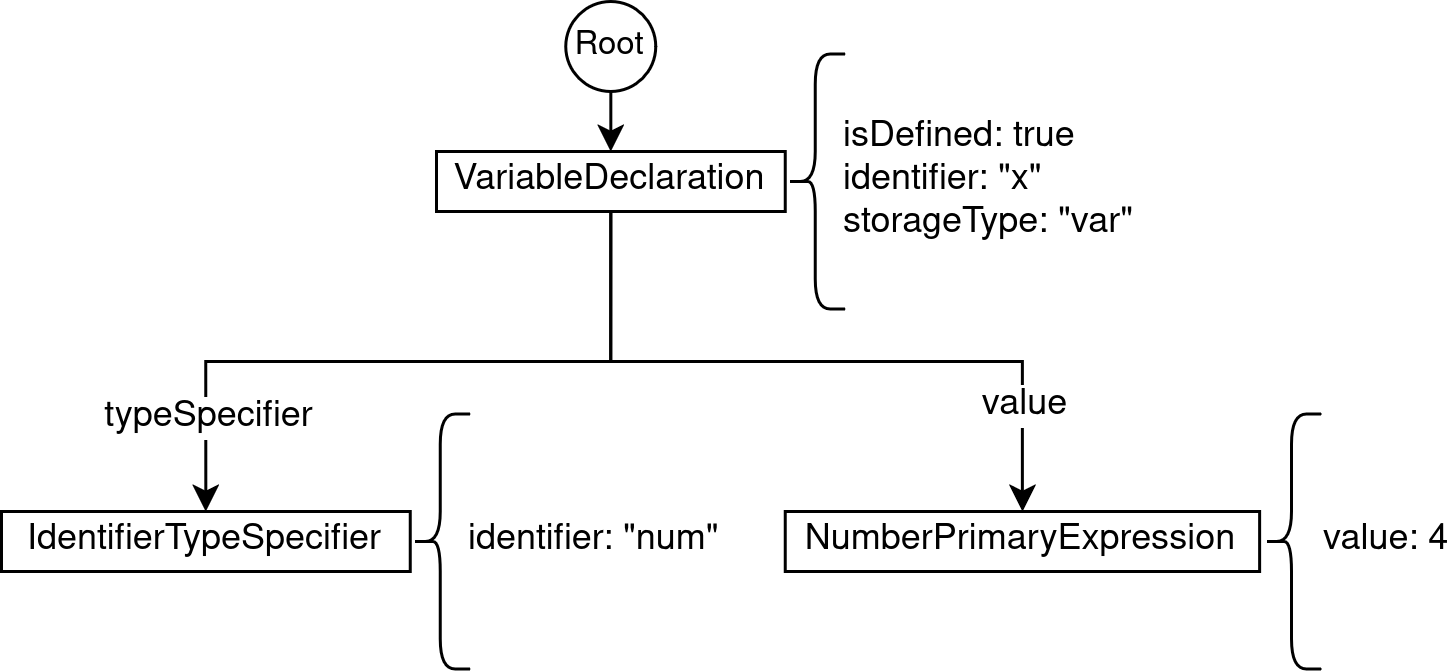
\includegraphics[scale=1]{./pics/AST.drawio}
	\caption{An AST produced by the statement \lstinline|var x: num = 4;|. The data in the brackets is in reality only defined and error checked during semantic analysis (see~\ref{sec:semantic-analysis}), but for the sake of clarity it is already provided here as to not cause confusion due to the missing metadata.}
	\label{fig:implementation:ast}
\end{figure}

\subsubsection{Utility provided by the AST}

In addition to providing a simplified abstraction of the original parse tree, individual \acrshort{ast} nodes also handle processing for several subsequent stages. Encapsulating these steps within a single class allows semantic analysis and type analysis to be efficiently layered and properly structured. This design is a core aspect of the compiler, as it centralizes data storage and ensures that the results of one processing stage directly influence subsequent stages.

For instance, if a node fails to successfully complete semantic analysis, the subsequent stages are automatically skipped. The node and any related parent structures are marked as faulty, allowing the compiler to handle errors gracefully without immediately crashing (see~\ref{sec:error-recovery} for a detailed explanation). Furthermore, the standardized and detailed structure of the \acrshort{ast} enables easy integration with other processing steps, as it stores or references all necessary information for specific parts of a program. This is particularly important during output generation (see~\ref{sec:output-generation}), where all existing information is required to accurately generate output code which logically adheres to the original program.

\section{Semantic Analysis}
\label{sec:semantic-analysis}
\setauthor{Luna Klatzer}

\section{Type Analysis}
\label{sec:type-analysis}
\setauthor{Luna Klatzer}

\section{Error recovery}
\label{sec:error-recovery}
\setauthor{Luna Klatzer}

The functionality of error recovery is integral to most modern compilers, as it allows the compiler to report multiple errors in a single compilation pass. Basic compilers often operate on an immediate fail-safe principle: upon encountering an error, the compilation process halts immediately to prevent the compiler from making incorrect assumptions about the program. While this approach ensures the integrity of the compilation process, it introduces a significant drawback. For large and complex programs, developers may need to repeatedly correct errors and recompile to uncover additional issues, leading to unnecessary delays and inefficiencies during the development process.

Given these issues, Kipper has implements its own error recovery algorithm into the semantic analysis which is able to recover from errors in given contexts and continue operation in following expressions or statements, which aren't associated with the original error.

\subsection{Error recovery algorithm}

\subsection{Special case: Syntax errors}

\section{Output Generation}
\label{sec:output-generation}
\setauthor{Lorenz Holzbauer}

\subsection{Introduction}

The Kipper compiler utilizes a modular architecture, allowing for the definition of custom targets and providing flexibility to accommodate various use cases. This modularity extends beyond basic configuration, enabling developers to specify target-specific features or behaviours. The modular design is achieved by dividing the compiler into two primary components: a frontend and a backend.

For comparison, the \acrshort{gcc} compiler achieves modularity by dividing its architecture into three components, as illustrated in Figure~\ref{fig:implementation:gcccompiler}. The frontend is responsible for verifying syntax and semantics, scanning the input, and performing type checking. It subsequently generates an intermediate representation (IR) of the code.

The middle-end then optimizes this intermediate representation, which is designed to be independent of the CPU target. Examples of middle-end optimizations include dead code elimination and detection of unreachable code. Finally, the backend takes the optimized intermediate code and generates target-dependent code. In the case of GCC, this involves generating assembly code.

\begin{figure}[h!]
	\centering
	\def\stackalignment{r}
	\stackunder{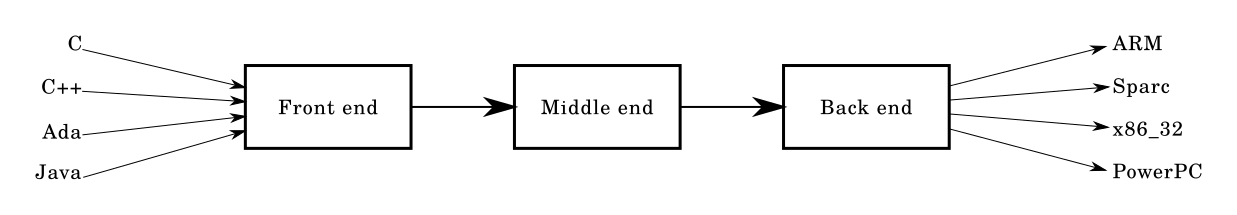
\includegraphics[scale=0.36]{./pics/Compiler_design}}{\scriptsize Source: \href{https://commons.wikimedia.org/wiki/File:Compiler_design.svg}{https://commons.wikimedia.org}}
	\caption{The design of the GCC compiler}
	\label{fig:implementation:gcccompiler}
\end{figure}

As of now, Kipper generates either TypeScript or JavaScript code as its output. The target language is specified in the Kipper CLI utility using the flag --target={js|ts}. If this flag is not provided, the default target is JavaScript.

Currently, Kipper does not include a middle-end component. This decision was made to avoid the additional complexity associated with implementing a full middle-end, as the resulting performance improvements in generated code would be only marginal. Instead, the frontend directly passes the \acrshort{ast} (Abstract Syntax Tree) to the backend. While Kipper does perform some post-analysis optimizations, these are presently limited to tree-shaking.

\subsection{Role of the AST in the output generation}

Kipper generally uses an \acrshort{ast} as the primary representation of the code from the input program. The \acrshort{ast} serves as a hierarchical structure that represents the program's source code. The root node of the \acrshort{ast} corresponds to the entire program, while each child node represents a specific construct such as a statement, scope, or other language feature.

Each node in the \acrshort{ast} contains the semantic data and type-related information of the corresponding statement, as well as a string representation of the original parser node. Additionally, every node includes a kind identification property—a unique, hard-coded number in the compiler—to uniquely identify the type of the node. This property aids in determining the type of construct, such as a declaration, an expression, or a statement.

Every node also maintains a list of child nodes, representing nested or dependent components of the construct. Once the \acrshort{ast} is fully constructed, it is wrapped and passed to the code generator for further processing.

\subsection{Algorithms used for Output Generation}

There is a plethora of algorithms available to generate code in the target language. They can be classified by their input data structure. Some algorithms need a tree-like \acrshort{ir}, others need a linear \acrshort{ir} structure.

\subsubsection{Linear Algorithms}

Linear algorithms are commonly employed when compiling high-level languages to machine code or bytecode. These algorithms treat the input as a flat, ordered sequence and process it sequentially. Intermediate representations (IR) are typically in the form of three-address code or static-single-assignment (SSA) form. Linear algorithms process the code one instruction at a time in sequence. Upon completion of an instruction, it is added to a list, which is eventually concatenated and written to the output file.

Three-address code consists of three operands and typically represents an assignment with a binary operator~\cite{wiki:threeaddress}. An instruction may have up to three operands, although fewer can also be used. In listing~\ref{lst:implementation:threeaddresscode}, the problem is divided into multiple instructions. This structure allows the compiler to easily translate the instructions into assembly language or bytecode, which share a similar format. Additionally, the compiler can identify unused code by determining whether a variable is referenced later in the code.

\begin{lstlisting}[language=TypeScript,caption=Three-address code,label=lst:implementation:threeaddresscode]
// Problem
x = (-b + sqrt(b^2 - 4*a*c)) / (2*a)

// Solution
t1 := b * b
t2 := 4 * a
t3 := t2 * c
t4 := t1 - t3
t5 := sqrt(t4)
t6 := 0 - b
t7 := t5 + t6
t8 := 2 * a
t9 := t7 / t8
x := t9
\end{lstlisting}

The Static Single-Assignment (SSA) form is an alternative intermediate representation in which each variable is assigned exactly once~\cite{wiki:singlestatic}. It is widely used in compilers such as \acrshort{gcc}. The primary advantage of SSA is that it simplifies the code and enhances the effectiveness of compiler optimizations.

In listing~\ref{lst:implementation:staticsingleassignmentform}, a variable \lstinline|y| is assigned twice. The first assignment is redundant. In SSA form, the compiler can identify that the assignment to \lstinline|y1| is unnecessary, as it is not used in the subsequent code. Optimizations improved by the use of SSA include dead-code elimination, constant propagation, and register allocation.

\begin{lstlisting}[language=TypeScript,caption=Static single-assignment form,label=lst:implementation:staticsingleassignmentform]
// Problem
y := 1
y := 2
x := y

// Solution
y1 := 1
y2 := 2
x1 := y2
\end{lstlisting}

\subsubsection{Tree-based Algorithms}

Tree-based algorithms are commonly employed in transpilers, as they allow the code to remain human-readable while preserving the general structure of the source code. This ensures that the structure of scopes and statements is maintained. Consequently, the components of the code are represented as nodes in a tree-like structure. Kipper adopts a bottom-up code generation algorithm, where a tree-walker recursively traverses the tree and generates the output starting from the most deeply nested node. This method was chosen for its ease of visualization and implementation, as well as the desire to retain human-readable and extendable source code without aggressive optimizations or transformations. This is not achievable with linear algorithms, which transform the code into either three-address code or static single-assignment form, leading to a loss of important contextual and structural information.

Tree-based code generation can be used to generate bytecode, which is then optimized and further compiled by a linear algorithm. However, tree-based algorithms have the limitation of enabling only local optimizations within the respective nodes. Additionally, they can be computationally expensive, particularly when dealing with complex input, due to the recursive nature of the tree-walking process. As a result, tree-based designs are not commonly employed in bytecode-generating compilers. However, \acrshort{gcc} uses a tree-based design in two of its language-independent IRs: GIMPLE and GENERIC~\cite{gcc:gimpletuples}.

\subsection{Generation Algorithm}

The output generation process in Kipper begins by setting up the target environment and generating any necessary requirements, as detailed in section~\ref{sec:requirements}. After completing the setup, the compiler iterates over the previously generated \acrshort{ast} nodes by invoking the \lstinline|translateCtxAndChildren| function for each node. This function recursively traverses the tree, generating code for each child node. Each node returns a string representing its output code, which is subsequently processed by its parent node. The process continues until the root node aggregates all generated strings and passes the final merged output to a function responsible for writing the code to a file.

This bottom-up processing approach ensures that the translation of child nodes is completed before their corresponding parent nodes are processed. Consequently, parent nodes can extract and integrate any required information from their child nodes. This methodology is particularly critical for complex structures, as these often depend on the embedded code generated by their children. The generated code is conveyed to the parent as an array of tokens, which represent the textual form of the output code.

The output generation process guarantees reliability because the \acrshort{ast} has already undergone validation for syntactic and semantic correctness during earlier compilation phases.

The implementation of this translation algorithm is presented in figure~\ref{fig:implementation:translationalgorithm}.

\begin{figure}[h!]
	\centering
	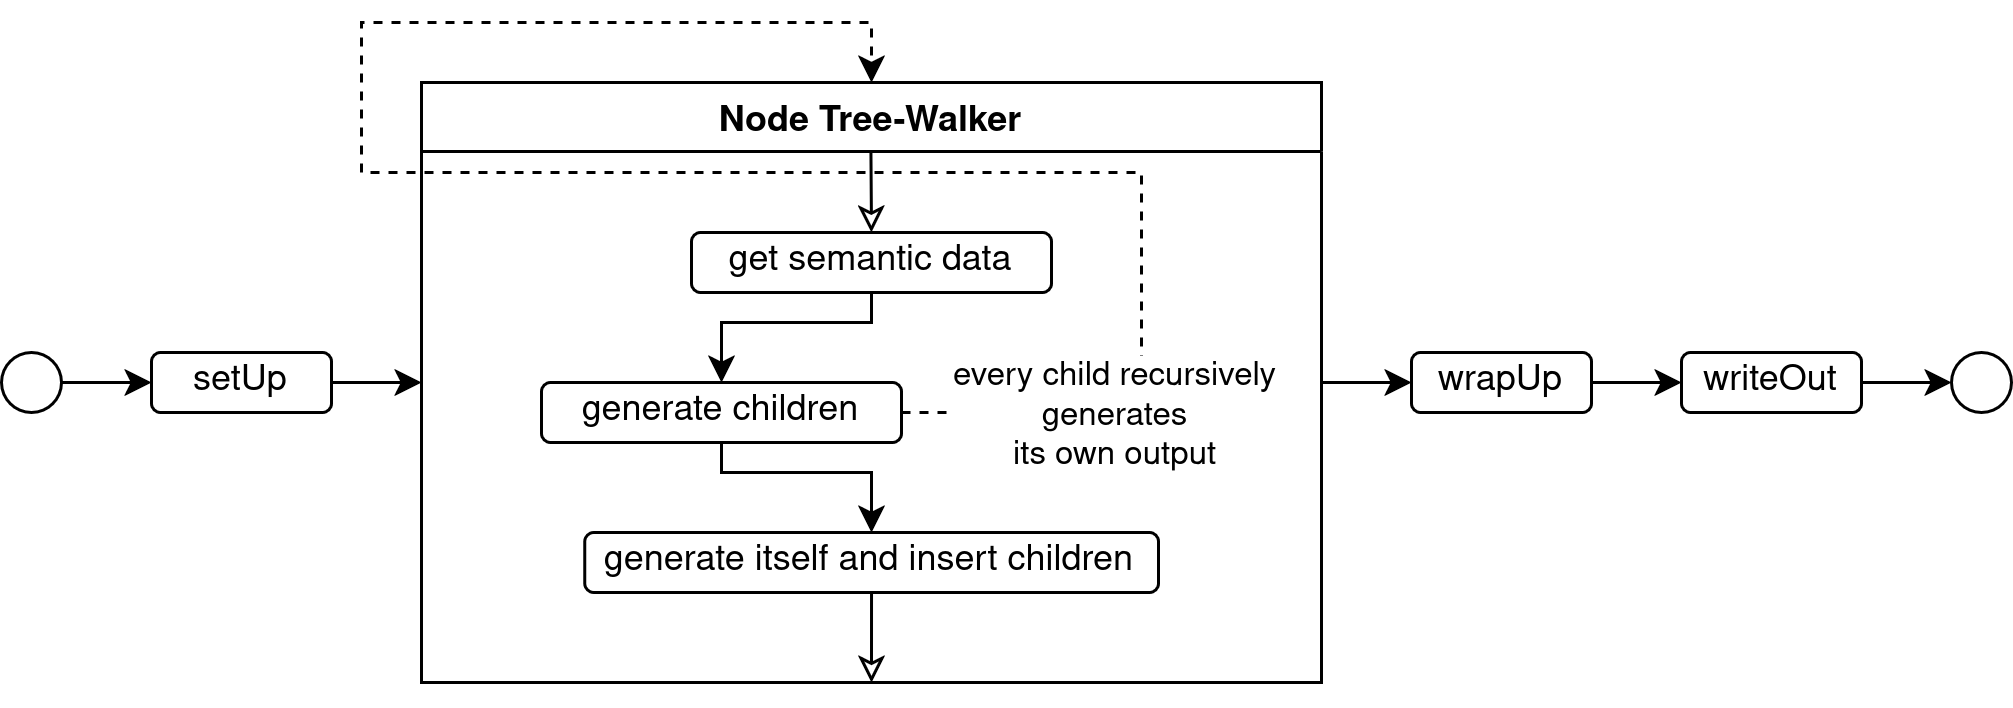
\includegraphics[scale=0.9]{./pics/Output-Generation.drawio}
	\caption{A simplified version of the tree-walker generation algorithm.}
	\label{fig:implementation:translationalgorithm}
\end{figure}

The code generation function of a node takes the node as an argument and retrieves its semantic and type-semantic data. This information is then used to translate the node's children, which are properties defined within the semantic data, into source code. The generated code fragments are concatenated into a single string array and returned. This process is demonstrated in listing~\ref{lst:implementation:instanceofgeneration}, where the translation of an \lstinline|instanceOf| expression is shown as an example.

\begin{lstlisting}[language=TypeScript,caption=The code generation function of a \lstinline|instanceOf| expression,label=lst:implementation:instanceofgeneration]
instanceOfExpression = async (node: InstanceOfExpression): ... => {
	const semanticData = node.getSemanticData();
	const typeData = node.getTypeSemanticData();
	const operand = await semanticData.operand.translateCtxAndChildren();
	const classType = TargetJS.getRuntimeType(typeData.classType);

    return [...operand, " ", "instanceof", " ", classType];
  };
\end{lstlisting}

The code generator functions for the individual nodes are implemented in the code generator class \lstinline|JavaScriptTargetCodeGenerator|. Due to the similarity between TypeScript and JavaScript, the TypeScript code generator extends the JavaScript code generator and overrides the functions that are unique to TypeScript. This eliminates duplicate code fragments.

\subsection{Target Requirements Generation}
\label{sec:requirements}

Kipper is designed to have a runtime that is as small as possible while still having all the needed functionality bundled in it. This means, that the compiler should only include functions and objects into the runtime, that are needed by the user. This aligns with our goal of keeping the compiler modular and minimal. Due to the removal of unused components in a process called "tree-shaking", the output code is kept small and efficient.

Kipper includes a range of built-in functions and features to support its runtime environment. These built-ins are organized and managed using a scoped approach. The global scope contains core runtime features that are always required, such as basic type handling and error reporting. Beyond the global scope, additional features are selectively included based on the specific requirements of the program being compiled.

\subsubsection{Conditional features}

Conditional features are runtime components that are included only when explicitly required by the program being compiled. These features can range from commonly used operations like match and slice to more specialized or program-specific utilities.

Unlike essential runtime components housed in the global scope, conditional features are added selectively based on an analysis of the program's structure and functionality. The decision to include conditional features occurs during the requirements generation phase. 

As the compiler traverses the \acrshort{ast}, it examines each node to determine whether a specific built-in function or runtime operation is invoked. If a feature like slice is used in the source code, it is flagged as necessary and included in the consolidated requirements list. This ensures that only the relevant components are integrated into the final runtime environment.

An example of a conditional feature would be the \lstinline|slice| function as shown in listing~\ref{lst:implementation:slicefunction}. 

\begin{lstlisting}[language=TypeScript,caption=The Slice Operation,label=lst:implementation:slicefunction]
var valid: str = "321";
print(valid[1:2]); // 2
\end{lstlisting}

This function takes an array as input and extracts a section starting from the index the first argument provides and ending at the index the second argument provides.

When the compiler encounters the slice operator, it registers the function as needed and therefore includes it into the output code. This process can be seen in listing~\ref{lst:implementation:sliceinternal}. 

The compiler calls the slice function in the \lstinline|BuiltInGenerator|. The abstract \lstinline|BuiltInGenerator| class is a collection of functions responsible for generating the code for the built-in functions in a specific target language. This means that each target language must have an individual implementation for each built-in function of Kipper within its output generator, which subsequently adds the corresponding code into the resulting program.

The generator in the listing~\ref{lst:implementation:sliceinternal} generates the required JavaScript code for the function by utilizing the built-in \lstinline|slice| function provided by standard JavaScript.

\begin{lstlisting}[language=TypeScript,caption=Slice in the JavaScript BuiltInGenerator,label=lst:implementation:sliceinternal]
async slice(funcSpec: InternalFunction): Promise<Array<TranslatedCodeLine>> {
	const signature = getJSFunctionSignature(funcSpec);
	const objLikeIdentifier = signature.params[0];
	const startIdentifier = signature.params[1];
	const endIdentifier = signature.params[2];

	return genJSFunction(
		signature,
		`{ return ${objLikeIdentifier} ? ${objLikeIdentifier}.slice(${startIdentifier}, ${endIdentifier}) : ${objLikeIdentifier}; }`,
	);
  }
\end{lstlisting}

The \lstinline|slice| function generated by the code generator as shown in listing~\ref{lst:implementation:sliceinternal} is represented in listing~\ref{lst:implementation:slicegenerated}. This function will be executed at runtime and perform the required operation, in this case slicing the given argument.

\begin{lstlisting}[language=TypeScript,caption=Slice in the target language TypeScript,label=lst:implementation:slicegenerated]
slice: function slice<T>(objLike: T, start: number | undefined, end: number | undefined): T {
	return objLike ? objLike.slice(start, end) : objLike;
},
\end{lstlisting}

\subsubsection{The global scope}

The global scope in programming represents the top-level execution context where variables, functions, and objects are accessible throughout the entire runtime environment unless explicitly restricted. In JavaScript, the global scope is particularly significant as it varies across runtime environments like browsers, Node.js, and Web Workers. This variability necessitates robust mechanisms for identifying and managing the global context to ensure compatibility across environments.

For example, JavaScript defines several global objects, such as window in browsers, global in Node.js, and self in Web Workers. Modern JavaScript unifies these under \lstinline|__globalScope|, a standardized global object that provides a consistent way to access the global scope regardless of the environment. However, not all environments support \lstinline|__globalScope|, which is why fallback mechanisms are often used.

The Kipper global scope contains all the runtime features that are required. It is important, that the global scope exists only once, therefore the program needs to check at runtime, if the scope already exists. This can be seen in listing~\ref{lst:implementation:globalscopelogic}. It first checks if \lstinline|__globalScope| is already defined and uses it if available. If not, it attempts to use \lstinline|globalThis|, the modern standard JavaScript global object. If \lstinline|globalThis| is not defined, it checks for window in browser environments, global in Node.js, or self in Web Workers. If none of these are defined, it falls back to an empty object. This ensures that the \lstinline|__globalScope| variable is always initialized, regardless of the environment, allowing consistent and safe access to the global scope.

\begin{lstlisting}[language=TypeScript,caption=Global Scope Logic,label=lst:implementation:globalscopelogic]
var __globalScope = typeof __globalScope !== "undefined" ? __globalScope :
    typeof globalThis !== "undefined" ? globalThis :
    typeof window !== "undefined" ? window :
    typeof global !== "undefined" ? global :
    typeof self !== "undefined" ? self : {};
\end{lstlisting}

\subsubsection{Internal functions}

Internal functions in Kipper serve as an essential part of the runtime, yet they are designed to remain hidden from the user-facing API. These functions provide support for various runtime operations and compiler processes but are not directly accessible or callable in the user's program. This ensures that the runtime environment remains clean and minimal while still delivering the required functionality.

An example of an internal function would be the \lstinline|assignTypeMeta| function, which adds metadata to a runtime type. This is useful for runtime type comparison and described in detail in chapter~\ref{subsec:builtintypes}. This function never gets exposed to the user but is called internally when an interface gets declared.

A key characteristic of internal functions is their dynamic inclusion in the runtime environment. During the requirements generation phase, the compiler identifies whether a program's functionality depends on any internal mechanisms. If so, the corresponding internal functions are included in the runtime.

\subsubsection{Requirements Generation}

The requirements generation process in Kipper begins during the compilation phase. As the compiler traverses the \acrshort{ast}, it analyses the nodes to determine the features needed by the program. This analysis produces a set of requirements, which are then used to configure the runtime environment. This works by using feature registration. If an AST node needs a certain feature, the reference is added to the program context by using the \lstinline|this.programCtx.addInternalReference| function. When a feature is added more once, all further additions get ignored, as the function is already available. After all the features are registered, the target generates the source code in the required language and inserts it into the output code.

\subsection{Differences between the Target Languages}

The implementation of a compiler or transpiler targeting multiple programming languages often requires handling the specific quirks and requirements of each target. As Kipper is a web development language, we target both TypeScript and JavaScript. Both languages share a common foundation but diverge significantly in their syntax rules, semantics, and type systems.

One of the primary challenges in supporting both JavaScript and TypeScript as target languages is their differing treatment of identifiers, reserved keywords, and type declarations. While JavaScript is dynamically typed and relatively permissive in terms of variable naming and usage, TypeScript enforces a stricter set of rules due to its static type-checking capabilities.

\subsubsection{Reserved Keywords}

Both JavaScript and TypeScript have a set of reserved keywords that cannot be used as identifiers. However, TypeScript introduces additional constraints by reserving type-related keywords, which are not present in JavaScript. For instance, class is a reserved keyword in both languages and cannot be used as a variable name. In contrast, TypeScript also reserves names like let, number, and other type names, making them invalid as variable or function names.

Kipper handles these reserved keywords by checking for them at compile time. The compiler compares against a hard-coded list of keywords and in case it finds one, it throws an \lstinline|ReservedIdentifierOverwriteError|. This list of keywords contains both the reserved words of JavaScript and TypeScript, as this minimizes redundancy and complexity. In addition to that, it also forces the developer to use sensible variable names, as JavaScript is quite lenient with it's reserved keywords. listing~\ref{lst:implementation:reservedkeywords} illustrates this.

\begin{lstlisting}[language=TypeScript,caption=Reserved Keywords in TS and JS,label=lst:implementation:reservedkeywords]
// Invalid in TypeScript
let let = 5;  // Error: Cannot use 'let' as an identifier
let number = 10;  // Error: Cannot use 'number' as an identifier

// Valid in JavaScript
var let = 5;  // No error
var number = 10;  // No error
\end{lstlisting}

\subsubsection{Type Annotations}

TypeScript introduces type annotations as part of its static type system. This means that while generating the TypeScript output, Kipper has to append type information in variable assignments, functions and lambdas. This works by overriding the JavaScript implementation of the code generator function and converting the AST-internal type of the node to a TypeScript type. 

Figures~\ref{fig:implementation:kipper-to-javascript-translation-example} and~\ref{fig:implementation:kipper-to-typescript-translation-example} shows the difference between the JavaScript code generator function and the TypeScript code generator function for variable assignments with the source example \lstinline|var x: num = 5;| being translated. In the code block that generates TypeScript, there are additional code tokens after the storage and the identifier that insert the type of the object into the output code.

\begin{figure}[h!]
	\centering
	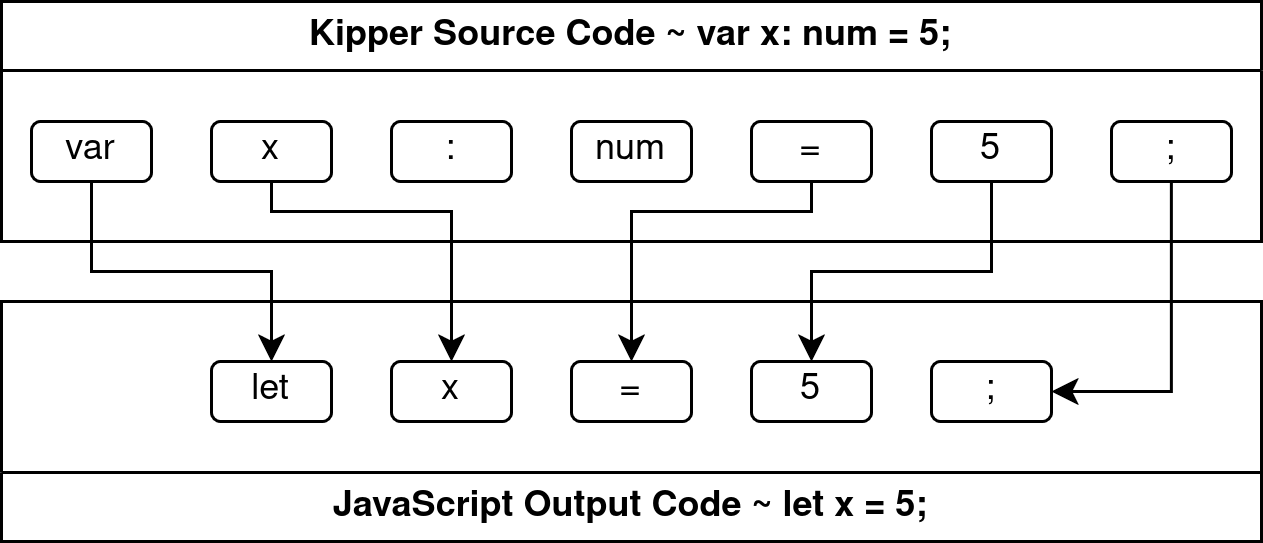
\includegraphics[scale=1.1]{./pics/Kipper-to-JavaScript-Translation-Example}
	\caption{The simplified translation process of the example \lstinline|var x: num = 5;| into JavaScript.}
	\label{fig:implementation:kipper-to-javascript-translation-example}
\end{figure}

\begin{figure}[h!]
	\centering
	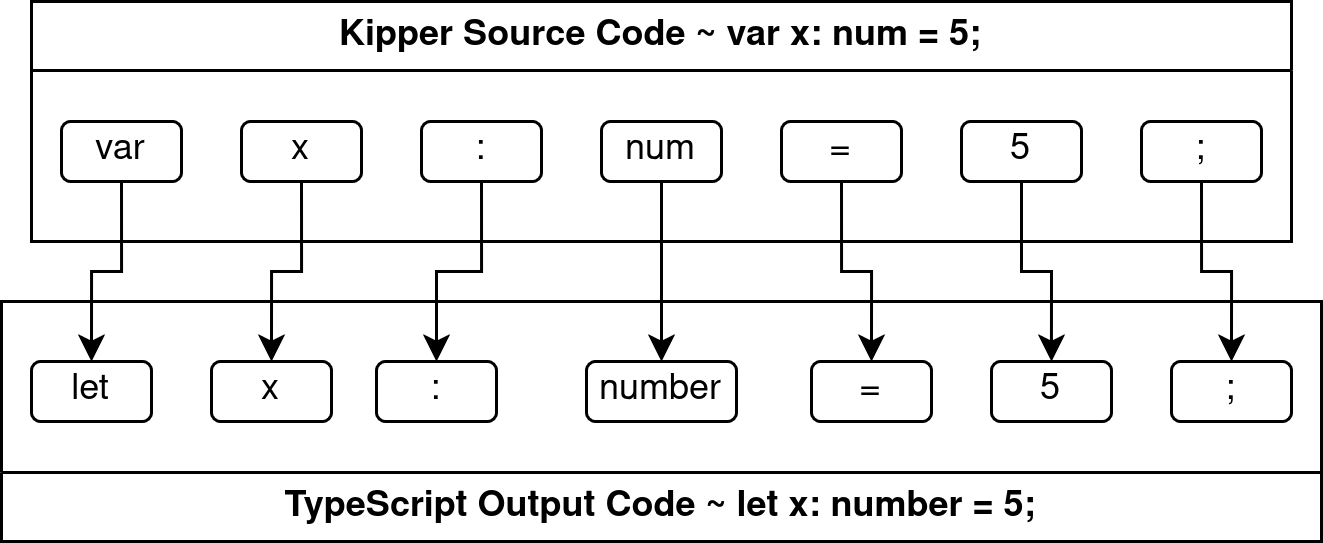
\includegraphics[scale=1.1]{./pics/Kipper-to-TypeScript-Translation-Example}
	\caption{The simplified translation process of the example \lstinline|var x: num = 5;| into TypeScript.}
	\label{fig:implementation:kipper-to-typescript-translation-example}
\end{figure}

Other code generators such as the ones for function declarations and lambdas behave similarly when taking type annotations into account.

\subsection{Stylistic Choices}

The syntax of Kipper is specifically designed to ease the transition of existing TypeScript and JavaScript developers to Kipper. Therefore it was important, to keep the output as similar to these languages as possible. We achieved this by adhering to the following principles.

\subsubsection{Human readable output}

The primary goal of Kipper's output generation is to produce code that mirrors human-written TS or JS as closely as possible. To achieve this, Kipper avoids unnecessary abstractions or layers that could obscure the intent of the code. For instance, variable names and function identifiers are preserved during \gls{transpilation} without introducing machine-generated names or hashing schemes. This contrasts with languages like CoffeeScript, where the output, while functional, often requires familiarity with the transpiler's conventions to interpret effectively.

\subsubsection{No Code Compression}

Kipper explicitly avoids code compression techniques such as minification or inlining that can hinder readability. While compression is useful in production environments to reduce payload size, it is opposed to the goals of Kipper, as it negatively impacts code readability.

\subsubsection{Standardized Style Format}

Kipper enforces a standardized style format for its output to ensure consistency and predictability. It uses two spaces for block-level indentation to maintain clarity and avoid confusion with tab-based formatting. Braces are explicitly used for block delimiters, and semicolons terminate statements, adhering to common TypeScript/JavaScript conventions.

\subsubsection{Scope Visibility}

A critical aspect of Kipper's design is the clear representation of scopes in the generated output. Kipper employs explicit declaration keywords such as \lstinline|let|, \lstinline|const|, and \lstinline|function| to discriminate variable and function scopes. Indentation and brace placement further enhance the visual hierarchy, making it easy to identify nested scopes and understand their boundaries. This approach contrasts with languages like Python, where indentation alone determines scope, or languages like Lua, where scope visibility may rely on implicit conventions.

\subsubsection{Editable Code}

One of Kipper's unique selling points is that its transpiled output is not just readable but also editable. Developers can treat the generated TS/JS code as if it were written manually, enabling seamless integration with existing projects. By making the output editable, Kipper empowers developers to tailor the transpiled code to their specific needs without relying solely on the original Kipper source.

\subsubsection{Comparison with other languages}

CoffeeScript aimed to simplify JavaScript syntax but often produced output that was hard to debug due to its reliance on non-standard conventions. Kipper avoids these pitfalls by aligning its syntax and output with established TypeScript/JavaScript practices. While TypeScript generates clean and maintainable JavaScript, it requires a compilation step that may introduce additional complexity. Kipper simplifies this process by direct \gls{transpilation} to both TypeScript and JavaScript, offering flexibility without sacrificing readability. Babel's output is highly optimized for compatibility but can be dense and difficult to modify. Kipper prioritizes maintainability over optimization, ensuring that the output remains approachable for developers.

\section{Integrated Runtime}
\label{sec:integrated-runtime}
\setauthor{Lorenz Holzbauer}

\subsection{Runtime Type implementations in other languages}
\label{chap:runtime-other-languages}

\subsubsection{Nominal Type Systems}

Nominal type systems are used in most modern object-orientated programming languages like Java and C\#. In these systems, types are identified by their unique names and can only be assigned to themselves. Additionally, two types are considered compatible, if one type is a subtype of the other one, as can bee seen in listing~\ref{lst:implementation:javanominaltyping}. Here a  \lstinline|Programmer| is an \lstinline|Employee|, but not the other way around. This means \lstinline|Programmer| instances have all the properties and methods an \lstinline|Employee| has while also having additional ones specific to \lstinline|Programmer|. The relationships are as such inherited, so \lstinline|SeniorDeveloper| is still an \lstinline|Employee| and a \lstinline|Programmer| at the same time. Even though the \lstinline|SeniorDeveloper| adds no new functionality to the \lstinline|Programmer|, it is not treated the same. Nominal typing improves code readability and maintainability, due to the explicit inheritance declaration. On the other hand, this increases code redundancy for similar or even identical but not related structures.

\begin{lstlisting}[language=Java,caption=Example of nominal typing in Java,label=lst:implementation:javanominaltyping]
class Employee {
	public float salary;
}

class Programmer extends Employee {
	public float bonus;
}

class SeniorDeveloper extends Programmer { }
\end{lstlisting}

\subsubsection{Structural Type Systems}

Structural type systems compare types by their structure. This means, if two differently named types have the same properties and methods, then they are the same type. An example of this would be OCaml, with its object subsystem being typed this way. Classes in OCaml only serve as functions for creating objects. In listing~\ref{lst:implementation:ocamlstructuraltyping} there is a function that requires a function \lstinline|speak| returning the type \lstinline|string|. Both the \lstinline|dog| object as well as the \lstinline|cat| object fulfill this condition, therefore both are treated equal. Most importantly, these compatibility checks happen at compile time, as OCaml is a static language. Structural typing allows for a lot of flexibility as it promotes code reuse. Furthermore it avoids explicit inheritance hierarchies.

\begin{lstlisting}[language=caml,caption=Example of structural typing in Ocaml,label=lst:implementation:ocamlstructuraltyping]
	let make_speak (obj : < speak : string >) =
	obj#speak

	let dog = object
	method speak = "Woof!"
	end

	let cat = object
	method speak = "Meow!"
	end

	let () =
	print_endline (make_speak dog);
	print_endline (make_speak cat);
\end{lstlisting}

\subsubsection{Duck Typed Systems - Duck Typing}

Duck Typing is the usage of a structural type system in dynamic languages. It is the practical application of the "Duck Test", therefore if it quacks like a duck, and walks like a duck, then it must be a duck. In programming languages this means that if an object has all methods and properties required by a type, then it is of that type. The most prominent language utilizing Duck Typing is TypeScript. As can be seen in listing~\ref{lst:implementation:javascriptducktyping}, the \lstinline|duck| and the \lstinline|person| have the same methods and properties, henceforth they are of the same type. The \lstinline|dog| object on the other hand does not implement the \lstinline|quack|function, which equates to not being a \lstinline|duck|. Duck typing simplifies the code by removing type constraints, while still encouraging polymorphism without complex inheritance.

\begin{lstlisting}[language=Typescript,caption=Example of duck typing in TypeScript,label=lst:implementation:javascriptducktyping]
interface Duck {
	quack(): void;
}

const duck: Duck = {
	quack: function () {
		console.log("Quack!");
	}
};

const person: Duck = {
	quack: function () {
		console.log("I am a person but I can quack!");
	}
};

const dog: Duck = {
	bark: function () {
		console.log("Woof!");
	}
}; // <- causes an error in the static type checker
\end{lstlisting}

Given that duck typing allows dynamic data to be easily checked and assigned to any interface, Kipper adopts a similar system to that of TypeScript but introduces notable differences in how interfaces behave and how dynamic data is handled. For instance, casting an \lstinline|any| object to an interface in Kipper will result in a runtime error if the object does not possess all the required members. In contrast, TypeScript permits such an operation without performing any type checks at runtime.

\subsection{Runtime Type Concept in Kipper}

As previously explained (see section~\ref{sec:type-system}) the Kipper programming language utilises a similar type system to TypeScript with static typing and a duck-typing approach to complex data and \acrshort{oop} structures. However, unlike TypeScript, we want to ensure full type safety at a runtime level and force the developer to specify the required types and handle edge cases, such as casts and type inference.

Using this approach Kipper allows untyped values, as is the case with the \lstinline|any| type that is often returned by requests or web elements, or dynamic values to be compared with types that have clearly defined boundaries, such as primitives, arrays, functions, classes, and interfaces, removing any ambiguities that could cause errors.

To allow this functionality, during code generation all user-defined interfaces are converted into runtime types that store the information needed to perform type checks, which form the basis of casts and strict type safety. These are then utilised alongside the built-in runtime types, such as \lstinline|num|, \lstinline|str| or \lstinline|obj|, to enable the compiler to add necessary checks and runtime references to any cast, match or typeof operation, guaranteeing that they are fully type-safe.

With the exception of interfaces, classes, and generics, types are primarily distinguished by their names. In these cases, type equality checks are performed using nominal comparisons, where the name acts as a unique identifier within the given scope e.g. type \lstinline|num| is only assignable to \lstinline|num|. For more complex structures, additional information—such as members or generic parameters—is also considered.

In the case of interfaces, the names and types of fields and methods are used as discriminators. These fields and methods represent the minimum blueprint that an object must implement to be considered compatible with the interface and thus "assignable". In this regard, Kipper adopts the same duck-typing approach found in TypeScript.

For generics, which include \lstinline|Array<T>| and \lstinline|Func<T..., R>|, the identifier is used alongside the provided generic parameters to determine assignability. This ensures that when one generic is assigned to another, all parameters must match. For instance, \lstinline|Array<num>| cannot be assigned to \lstinline|Array<str>"|and vice versa, even if their overall structure is identical.

For user-defined classes, the compiler relies on the prototype to serve as the discriminator. In practice, this behaviour is similar to that of primitives, as different classes cannot be assigned to each other.

\subsection{Base Type for the Kipper Runtime}
\label{subsec:basetype}

In practice, all user-defined and built-in types inherit from a basic \lstinline|KipperType| class in the runtime environment. This class is a simple blueprint of what a type could do and what forms a type may take on. A simple version of such a class can be seen in listing~\ref{lst:implementation:runtimetypestructure}.

\begin{lstlisting}[language=TypeScript,caption=The structure of a runtime type,label=lst:implementation:runtimetypestructure]
	class KipperType {
		constructor(name, fields, methods, baseType = undefined, customComparer = undefined) {
			this.name = name;
			this.fields = fields;
			this.methods = methods;
			this.baseType = baseType;
			this.customComparer = customComparer;
		}

		accepts(obj) {
			if (this === obj) return true;
			return obj instanceof KipperType && this.customComparer ? this.customComparer(this, obj) : false;
		}
	}
\end{lstlisting}

As already mentioned types primarily rely on identifier checks to differentiate themselves from other types. Given though that there are slight differences in how types operate, they generally define themselves with what they are compatible using a comparator function. This comparator is already predefined for all built-ins in the runtime library and any user structures build on top of the existing rules established in the library.

Type \lstinline|any| is an exception and is the only type that accepts any value you provide. However, assigning "any" to anything other than \lstinline|any| is forbidden and it is necessary to cast it to a different type in order to use the stored value. By  \lstinline|any| is as useless as possible, in order to force the developer into typechecking it.

Furthermore, classes are also exempt from this comparator behaviour, as classes behave like a value during runtime and provide a prototype which can simply be used to check if an object is an instance of that class.

\subsection{Built-in Types for the Kipper Runtime}
\label{subsec:builtintypes}

Built-in runtime types serve as the foundation of the type system and make up the parts of more complex constructs like interfaces. Built-in runtime types are compared at runtime by comparing their references, as they are uniquely defined at the start of the output code and available in the global scope. The implementations of such structures can be seen in listing~\ref{lst:implementation:builtinruntimetypes}.

\begin{lstlisting}[language=TypeScript,caption=Examples for the built-in runtime types,label=lst:implementation:builtinruntimetypes]
	const __type_any =
	new KipperType("any", undefined, undefined);

	const __type_undefined =
	new KipperType("undefined", undefined, undefined, undefined, (a, b) => a.name === b.name);

	const __type_str =
	new KipperType("str", undefined, undefined, undefined, (a, b) => a.name === b.name);
\end{lstlisting}

In addition to the core primitive types—such as \lstinline|bool|, \lstinline|str|, \lstinline|num|, and others—there are built-in implementations for generic types, including \lstinline|Array<T>| and  \lstinline|Func<T..., R>|. These additionally define their generic parameters which generally default to a standard \lstinline|any| type as can be seen in listing~\ref{lst:implementation:genericbuiltintypes}.

\begin{lstlisting}[language=Typescript,caption=Generic built-in types,label=lst:implementation:genericbuiltintypes]
const __type_Array = new KipperGenericType("Array", undefined, undefined, {T: __type_any});
const __type_Func = new KipperGenericType("Func", undefined, undefined, {T: [], R: __type_any});
\end{lstlisting}

As can be seen in listing~\ref{lst:implementation:genericbuiltintypes}, generic types are implemented using a special \lstinline|KipperGenericType| class. This class, shown in listing~\ref{lst:implementation:generickippertype}, extends the \lstinline|KipperType| and includes an additional field for generic arguments. Most importantly, it includes the method \lstinline|changeGenericTypeArguments|. which allows for modifying a type's generic arguments at runtime. It is used in lambda and array definitions, where the built-in generic runtime type is used and then modified to represent the specified generic parameters. When for example an array is initialized, it first gets assigned the default \lstinline|Array<any>| runtime type, which is then modified by the  \lstinline|changeGenericTypeArguments| method to create the required type, such  \lstinline|Array<num>|. Arrays for example use the specified type for their elements, whilst functions require a return type as well as an array of argument types. The \lstinline|Func<T..., R>| type on the other hand is used by lambda definitions, which are user-defined functions with a specific return type and arguments without a name \ref{lst:implementation:generickippertype}.

\begin{lstlisting}[language=Typescript,caption=Generic Kipper Type,label=lst:implementation:generickippertype]
class KipperGenericType extends KipperType {
	constructor(name, fields, methods, genericArgs, baseType = null) {
		super(name, fields, methods, baseType);
		this.genericArgs = genericArgs;
	}
	isCompatibleWith(obj) {
		return this.name === obj.name;
	}
	changeGenericTypeArguments(genericArgs) {
		return new KipperGenericType(
		this.name,
		this.fields,
		this.methods,
		genericArgs,
		this.baseType
		);
	}
}
\end{lstlisting}

\subsection{Runtime Errors}

Other built-ins include error classes, which are used in the error handling system to represent runtime errors caused by invalid user operations. The base \lstinline|KipperError| type has a name property and extends the target language's error type as can be seen in listing~\ref{lst:implementation:kippererrortypes}. Additional error types inherit this base type and extend it with additional error information. For instance, the  \lstinline|KipperIndexError| is used whenever an index was out of bounds.

\begin{lstlisting}[language=Typescript,caption=Kipper error types,label=lst:implementation:kippererrortypes]
class KipperError extends Error {
	constructor(msg) {
		super(msg);
		this.name = "KipError";
	}
}

class KipperIndexError extends KipperError {
	constructor(msg) { 
		super(msg); 
		this.name = 'KipIndexError'; 
	} 
}
\end{lstlisting}

\subsection{Runtime Generation for Interfaces}

Unlike TypeScript, in Kipper all interfaces possess a runtime counterpart, which stores all the required information to verify type compatibility during runtime. This process is managed by the Kipper code generator, which adds custom type instances to the compiled code that represent the structures of the user-defined interfaces with all its methods and properties including their respective types.

Now take for example the given interfaces presented in listing~\ref{lst:implementation:inputinterface-car} and~\ref{lst:implementation:inputinterface-person}.

\begin{lstlisting}[language=Typescript,caption=Example interface \lstinline|Car| in the Kipper language,label=lst:implementation:inputinterface-car]
interface Car {
	brand: str;
	honk(volume: num): void;
	year: num;
}
\end{lstlisting}

\begin{lstlisting}[language=Typescript,caption=Example interface \lstinline|Person| in the Kipper language including a reference to a different interface,label=lst:implementation:inputinterface-person]
interface Person {
	name: str;
	age: num;
	car: Car;
}
\end{lstlisting}

At compile time, the generator function iterates over the interface's members and differentiates between properties and methods. The function keeps separate lists of already generated runtime representations for properties and methods.

If it detects a property, the type and semantic data of the given property is extracted. When the property's type is a built-in type, the respective runtime type already provided by the Kipper runtime library is used. If not, we can assume the property's type is a reference to another type structure, which will be simply referenced in our new type structure. This data is stored in an instance of \lstinline|__kipper.Property|, which is finally added to the list of properties in the interface.

In case a method is detected, the generator function fetches the return type and the method's name. If the method has any arguments, the name and type of each argument also gets evaluated and then included in the definition of the \lstinline|__kipper.Method|. After that, it gets added to the interface as well and is stored in its own separate method list.

Translating the interface \lstinline|Car| shown in listing~\ref{lst:implementation:inputinterface-car} would result in an output runtime code identical to that in listing~\ref{lst:implementation:runtimeinterface-car} and translating \lstinline|Person| would result in the code as presented in listing~\ref{lst:implementation:runtimeinterface-person}.

\begin{lstlisting}[language=Typescript,caption=The runtime representation of the example interface \lstinline|Car|,label=lst:implementation:runtimeinterface-car]
const __intf_Car = new __kipper.Type(
	"Car",
	[
		new __kipper.Property("brand", __kipper.builtIn.str),
		new __kipper.Property("year", __kipper.builtIn.num),
	],
	[
		new __kipper.Method("honk", __kipper.builtIn.void,
			[
				new __kipper.Property("volume", __kipper.builtIn.num),
			]
		),
	]
);
\end{lstlisting}

\begin{lstlisting}[language=Typescript,caption=The runtime representation of the example interface \lstinline|Person|,label=lst:implementation:runtimeinterface-person]
const __intf_Person = new __kipper.Type(
	"Person",
	[
		new __kipper.Property("name", __kipper.builtIn.str),
		new __kipper.Property("age", __kipper.builtIn.num),
		new __kipper.Property("car", __intf_Car),
	],
	[]
);
\end{lstlisting}

As shown in listing~\ref{lst:implementation:runtimeinterface-car} and listing~\ref{lst:implementation:runtimeinterface-person}, the properties and methods of an interface are encapsulated within a \lstinline|KipperType| instance, identified by the  \lstinline|__intf_| prefix. The code for this runtime interface is included directly in the output file, where it can be accessed by any functionality that requires it. To reference the generated interface, the compiler maintains a symbol table that tracks all defined interfaces. The code generator then inserts runtime references to these interfaces wherever necessary.

Notable usages for runtime type-checking include the \lstinline|matches| operator (see section \ref{subsec:matches}) and the \lstinline|typeof| operator (see section \ref{subsec:typeof}).

\subsection{Matches Operator for Interfaces}
\label{subsec:matches}

There are multiple approaches for comparing objects at runtime. One method is comparison by reference, which is implemented using the \lstinline|instanceof| operator. This method determines that an object is an instance of a class if there is a reference to that class, leveraging JavaScript's prototype system.

Another approach is comparison by structure, where two objects are considered equal if they share the same structure, meaning they have the same properties and methods. Kipper supports both methods of comparison. Reference-based comparison is implemented via the \lstinline|instanceof| operator and is exclusively used for class comparisons. Structural comparison, referred to as "matching", is applied to primitives and interfaces. 

Structural comparisons are implemented using the \lstinline|matches| operator as given in listing~\ref{lst:implementation:matchesoperator}.

\begin{lstlisting}[language=Typescript,caption=The Kipper matches operator,label=lst:implementation:matchesoperator]
interface Y {
	v: bool;
	t(gr: str): num;
}

interface X {
	y: Y;
	z: num;
}

var x: X = {
	y: {
		v: true,
		t: (gr: str): num -> {
			return 0;
		}
	},
	z: 5
};

var res: bool = x matches X; // -> true
\end{lstlisting}

As can be seen in listing~\ref{lst:implementation:matchesoperator}, the matches operator can compare interfaces by properties and methods. It takes two arguments, an object and a type which it should match. Properties are compared recursively and methods are compared by name, arguments and return type.

Comparison works by iterating over the methods and properties. When iterating over the properties, it checks for the property's name being present in the type it should check against. The order of properties does not matter. When the name is found, it checks for type equality. This checking is done using the aforementioned runtime types and nominal type comparison. In case a non-primitive is detected as the properties type, the matches function will be recursively executed on non-primitives.

This property match algorithm is implemented as given in listing~\ref{lst:implementation:matchesproperty}.

\begin{lstlisting}[language=Typescript,caption=Matches operator property comparison,label=lst:implementation:matchesproperty]
for (const field of pattern.fields) {
  const fieldName = field.name;
  const fieldType = field.type;

  if (!(fieldName in value)) {
    return false;
  }

  const fieldValue = value[fieldName];
  const isSameType = __kipper.typeOf(fieldValue) === field.type;

  if (primTypes.includes(field.type.name) && !isSameType) {
    return false;
  }

  if (!primTypes.includes(fieldType.name)) {
    if (!__kipper.matches(fieldValue, fieldType)) {
      return false;
    }
  }
}
\end{lstlisting}

After checking the properties, the matches expression iterates over the methods. It first searches for the method name in the target type. If found, it compares the return type. Then each argument is compared by name. As the methods signatures need to be exactly the same, the amount of parameters is compared as well.

\begin{lstlisting}[language=Typescript,caption=Matches operator method comparison,label=lst:implementation:matchesmethod]
for (const field of pattern.methods) {
  const fieldName = field.name;
  const fieldReturnType = field.returnType;
  const parameters = field.parameters;

  if (!(fieldName in value)) {
    return false;
  }

  const fieldValue = value[fieldName];
  const isSameType = fieldReturnType === fieldValue.__kipType.genericArgs.R;

  if (!isSameType) {
    return false;
  }

  const methodParameters = fieldValue.__kipType.genericArgs.T;

  if (parameters.length !== methodParameters.length) {
    return false;
  }

  let count = 0;
  for (let param of parameters) {
    if (param.type.name !== methodParameters[count].name) {
      return false;
    }
    count++;
  }
}
\end{lstlisting}

When none of these conditions are false, the input object matches the input type and they can be seen as compatible.

\subsection{Typeof Operator}
\label{subsec:typeof}

In the Kipper programming language, the \lstinline|typeof| operator is used to get the type of an object at runtime. This operator can be used to check if a variable or expression is of a particular type, such as a string, number, boolean, etc. Most commonly, it is used to check for null and undefined objects, to avoid type errors when an object is of unknown type. The returned type object can be compared by reference to check for type equality. As can bee seen in listing~\ref{lst:implementation:typeofoperator}, the parantheses are optional. We decided to allow both syntax styles, due to our goal of being similar to TypeScript and JavaScript, which both implement it the same way.

\begin{lstlisting}[language=Typescript,caption=Typeof operator used to determine the type of an input expression,label=lst:implementation:typeofoperator]
typeof 49; // "__kipper.builtIn.num"
typeof("Hello, World!"); // "__kipper.builtIn.str"
\end{lstlisting}

The  \lstinline|typeof| operator in Kipper mirrors the functionality of TypeScript and JavaScript, but with enhancements tailored to Kipper's type system. Unlike JavaScript, where the  \lstinline|typeof null| returns \lstinline|object| due to historical reasons, Kipper correctly identifies  \lstinline|null| as  \lstinline|__kipper.builtIn.null|.

At runtime, the provided object is checked for it's type using the target languages type features. A part of this process can be seen in figure~\ref{fig:implementation:typeofimplementation}. The primitive types return their respective \lstinline|KipperRuntimeType|. Objects are a special case, as they can either be null, an array, a class or an object, for example one that implements an interface.

\begin{figure}[h!]
	\centering
	\def\stackalignment{r}
	\stackunder{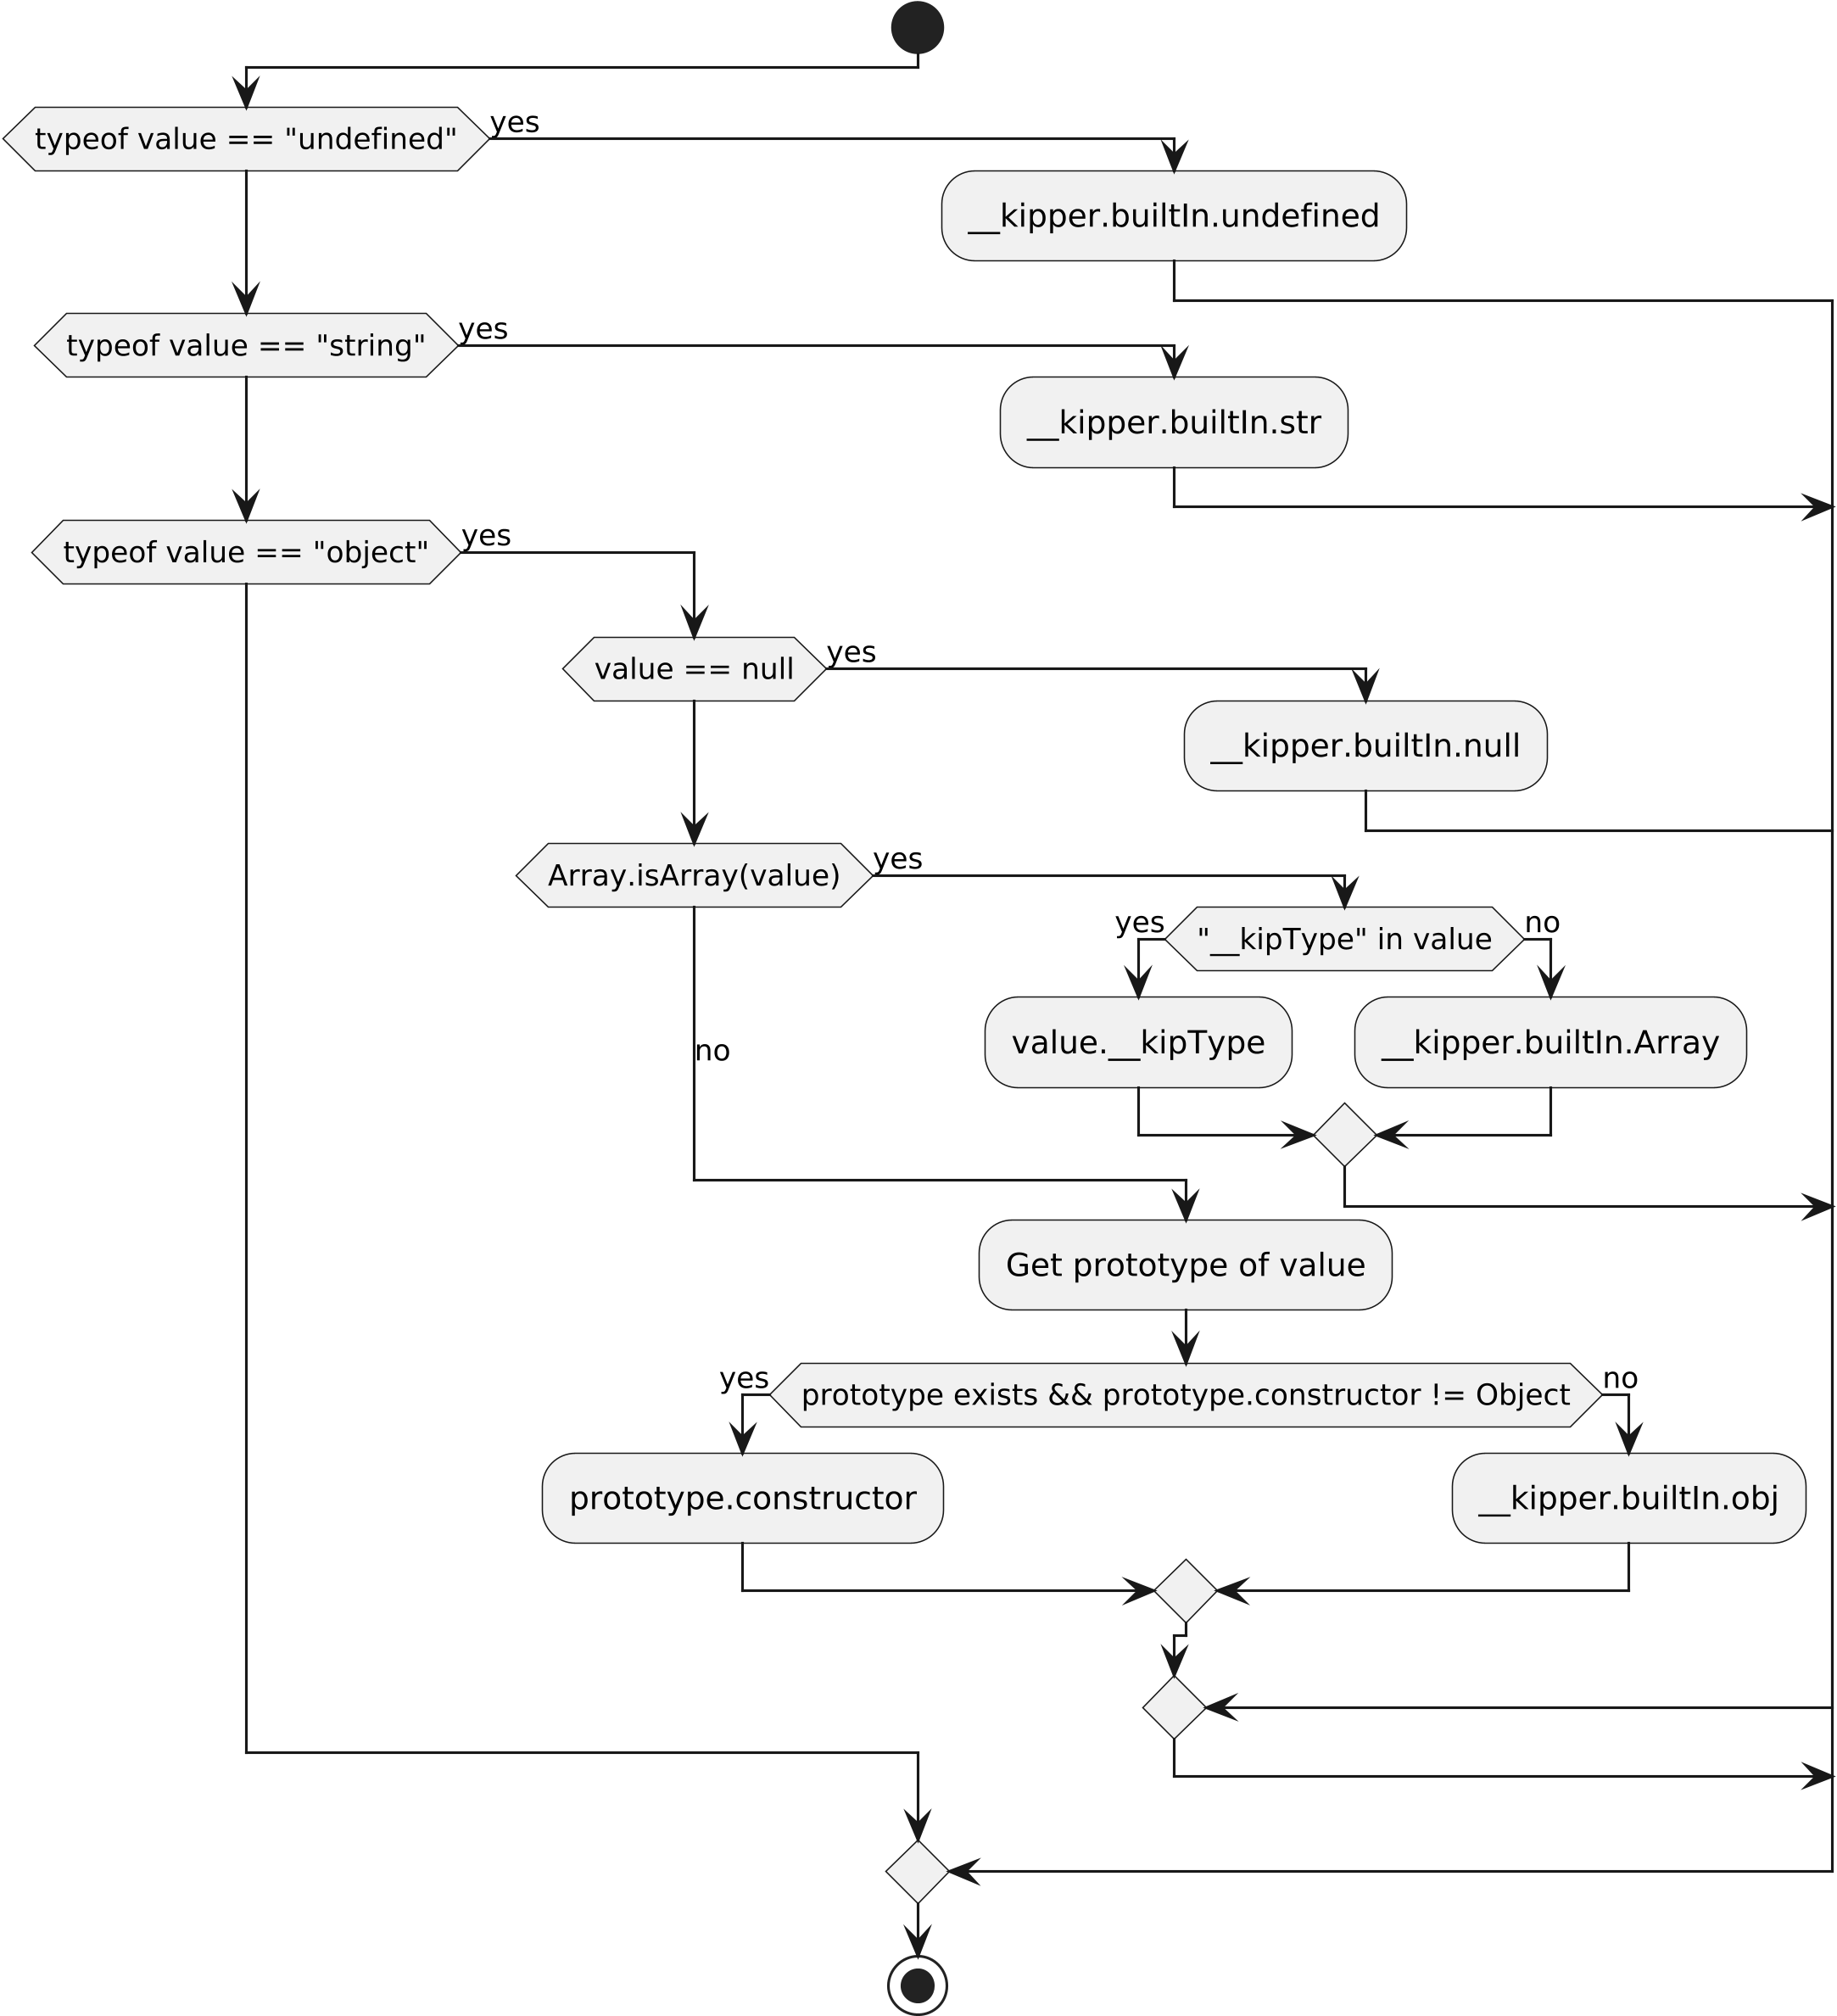
\includegraphics[scale=0.25]{./pics/typeOfImplementation}}{}
	\caption{Logical implementation of the typeof operator in TypeScript}
	\label{fig:implementation:typeofimplementation}
\end{figure}


Although linguistically quite similar, the \lstinline|typeof| operator in the type declaration of a variable works fundamentally different~\ref{lst:implementation:typeoftypespecifier}. It is called \lstinline|TypeOfTypeSpecifier| and it evaluates the type of a variable at compile time.

\begin{lstlisting}[language=Typescript,caption=Specifying the type based on a reference variable, label=lst:implementation:typeoftypespecifier]
var t: num = 3;
var count: typeof(t) = 4;
\end{lstlisting}

%%% Local Variables:
%%% mode: LaTeX
%%% TeX-master: "../thesis"
%%% End:


\begin{spacing}{1}
\chapter{Compiler Reference}\label{chapter:compiler_ref}
\end{spacing}
\setauthor{Lorenz Holzbauer}

\section{Compiler API}
\label{sec:compiler_api}

The Kipper Compiler API provides the necessary functionality to compile Kipper source code into JavaScript or TypeScript. The main entry points into the API are the \lstinline|KipperCompiler| class and the \lstinline|KipperProgramContext| class.

\subsection{Initializing the Compiler}
\label{subsec:compiler_init}

To compile Kipper code, an instance of \lstinline|KipperCompiler| must be created. The compiler requires a logger instance and an optional configuration object.

\begin{lstlisting}[language=Typescript, caption=Initializing the Kipper Compiler, label=lst:compiler_initialization]
const logger = new Kipper.KipperLogger((level, msg) => {
	console.log(`[${Kipper.getLogLevelString(level)}] ${msg}`);
});

const compiler = new Kipper.KipperCompiler(logger, {});
\end{lstlisting}

The logger instance provides error reporting functionality, making it an essential part of the compilation process.

\subsection{Compiling Kipper Code}
\label{subsec:compiling}

Once the compiler is initialized, it can be used to transpile Kipper code into JavaScript or TypeScript. The \lstinline|compile| method takes the source code as a string and a configuration object specifying the compilation target.

\begin{lstlisting}[language=Typescript, caption=Compiling Kipper Code to JavaScript, label=lst:compile_example]
const result = await compiler.compile(
	`print("Hello world!");`,
	{ target: new KipperJS.TargetJS() }
);
const jsCode = result.write();

// Execute the compiled JavaScript
eval(jsCode);
\end{lstlisting}

The compilation result is an object containing the generated JavaScript or TypeScript code, which can be executed or written to a file.

\subsection{Compilation Options}
\label{subsec:compilation_options}

The \lstinline|compile| method accepts a configuration object that allows customization of the compilation process. The most important options are:

\begin{itemize}
	\item \lstinline|target|: Specifies the output language. Available targets are \lstinline|TargetJS| for JavaScript and \lstinline|TargetTS| for TypeScript.
	\item \lstinline|filename|: Specifies the filename of the generated code
	\item \lstinline|optimisationOptions|: Currently
	\lstinline|optimiseInternals| and \lstinline|optimiseBuiltIns| are available. They can be enabled by setting them to \lstinline|true|
\end{itemize}

\section{Target API}
\label{sec:target_api}

The Kipper compiler supports multiple compilation targets, allowing the transpilation of Kipper code into different languages. Developers can extend Kipper by implementing custom targets.

\subsection{Using Predefined Targets}
\label{subsec:using_targets}

Kipper provides predefined targets for JavaScript and TypeScript. These can be used as follows:

\begin{lstlisting}[language=Typescript, caption=Using Compilation Targets, label=lst:using_targets]
const jsTarget = new KipperJS.TargetJS();
const tsTarget = new KipperJS.TargetTS();
\end{lstlisting}

\subsection{Creating Custom Targets}
\label{subsec:custom_targets}

To create a custom target, a new class must extend \lstinline|KipperTarget| and implement the \lstinline|transpile| method.

\begin{lstlisting}[language=Typescript, caption=Creating a Custom Compilation Target, label=lst:custom_target]
class CustomTarget extends Kipper.KipperTarget {
	transpile(ast) {
		// Custom transpilation logic
		return "// Transpiled code";
	}
}
\end{lstlisting}

This allows for custom language backends beyond JavaScript and TypeScript.

\section{CLI Interface}
\label{sec:cli_interface}

The Kipper CLI provides a command-line interface for compiling Kipper code. The CLI is available via the \lstinline|@kipper/cli| package.

\subsection{Installing the CLI}
\label{subsec:cli_installation}

To install the Kipper CLI, use the following command:

\begin{lstlisting}[language=bash, caption=Installing Kipper CLI, label=lst:cli_install]
npm install @kipper/cli
\end{lstlisting}

This installs Kipper in the current NPM project. To install Kipper globally, use the \lstinline|-g| flag. This may require superuser privileges, depending on the installation location.

\subsection{Compiling a File}
\label{subsec:cli_compile}

To compile a Kipper source file, use the \lstinline|kipper compile| command:

\begin{lstlisting}[language=bash, caption=Compiling a Kipper File, label=lst:cli_compile]
kipper compile source.kip --target js
\end{lstlisting}

This command transpiles \lstinline|source.kip| to JavaScript. It is possible to specify the option \lstinline|--target=ts| to switch to the TypeScript target. When no target option is specified, the default target is JavaScript.

\subsection{Running a Kipper Program}

To run a Kipper source file, use the \lstinline|kipper run| command:

\begin{lstlisting}[language=bash, caption=Running a Kipper File, label=lst:cli_run]
	kipper run source.kip
\end{lstlisting}

This command transpiles to the specified target and then executes the code.

\subsection{Creating a New Project}
\label{subsec:cli_new_project}

To create a new Kipper project, use:

\begin{lstlisting}[language=bash, caption=Creating a New Kipper Project, label=lst:cli_new_project]
kipper new my_project
\end{lstlisting}

This generates a new project with the necessary configuration files.

%%% Local Variables:
%%% mode: LaTeX
%%% TeX-master: "../thesis"
%%% End:

\begin{spacing}{1}
\chapter{Demo \& Showcase}\label{chapter:demo}
\end{spacing}
\setauthor{Lorenz Holzbauer}

This chapter explores various sample use cases for Kipper to showcase its capabilities and demonstrate the environments in which it can be utilized. To keep things concise and focused, the examples provided will cover simple scenarios. More complex applications are beyond the scope of this paper, but can be explored in further documentation (see \nameref{chapter:appendix_b} for further details).

\section{Example Program}
\setauthor{Lorenz Holzbauer}

Listing \ref{lst:demo:isprime} demonstrates the computation of the prime factors of a given number using Kipper. The program is given a number, determines the prime factors and prints the result.

\begin{lstlisting}[language=Kipper,caption=A basic programs that determines the prime factors of an integer, label=lst:demo:isprime]
def primeFactors(n: num) -> void {
	while (n % 2 == 0) {
		print(2);
		n /= 2;
	}
	
	for (var i: num = 3; i * i <= n; i += 2) {
		while (n % i == 0) {
			print(i);
			n /= i;
		}
	}
	
	if (n > 2) {
		print(n);
	}
}

primeFactors(18);
\end{lstlisting}

\section{Working example using CLI}
\setauthor{Lorenz Holzbauer}

Kipper provides a command-line interface (CLI) that allows users to compile and execute programs directly from the terminal. To run the above example using the CLI, the following steps are required:

\begin{enumerate}
	\item Install the Kipper CLI globally using npm: \lstinline|npm install -g @kipper/cli|
	\item Save the Kipper source code in a file, e.g., \texttt{prime.kip}.
	\item Compile and execute a Kipper file: \lstinline|kipper run prime.kip|
\end{enumerate}

After execution, the prime factors of the given number are printed to the console.

\section{Working example in the web}
\setauthor{Lorenz Holzbauer}

Kipper can also be run in the browser using the \texttt{@kipper/web} package. Listing \ref{lst:demo:kipperbrowser} demonstrates how to include Kipper in an HTML file and execute the same prime factorization program.

\begin{lstlisting}[language=HTML,caption=Running Kipper in the browser, label=lst:demo:kipperbrowser]
<!DOCTYPE html>
<head>
	<title>Kipper Demo</title>
	<script src="https://cdn.jsdelivr.net/npm/@kipper/web@latest
	/kipper-standalone.min.js"></script>
</head>
<body>
	<script type="module">
		const logger = new Kipper.KipperLogger((level, msg) => {
			console.log(`[${Kipper.getLogLevelString(level)}] ${msg}`);
		});
		
		const compiler = new Kipper.KipperCompiler(logger, {});
		
		const code = ''; // Replace with prime.kip
		
		compiler.compile(
			code, 
			{ target: new KipperJS.TargetJS() }
		).then((result) => {
			const jsCode = result.write();
			eval(jsCode);
		});
	</script>
</body>
\end{lstlisting}

When opened in a browser, this file will execute the compiled JavaScript version of the prime factorization program, displaying the results in the browser console.

\section{Working example using Node.js}
\setauthor{Lorenz Holzbauer}




\begin{spacing}{1}
\chapter{Conclusion \& Future}
\end{spacing}
\section{Future}
\label{sec:future}
\setauthor{Lorenz Holzbauer}

Currently, Kipper caters primarily to web developers by providing seamless integration with the TS and JS ecosystems. This focus aligns well with the popularity of JavaScript on both the client and server sides. However, the web development landscape is rapidly evolving, and developers are increasingly seeking high-performance solutions.

\subsection{WebAssembly Support}
%https://webassembly.org/
%https://wasmer.io/

WebAssembly is an open standard that enables high-performance, portable code execution across diverse environments, including browsers, servers, and embedded systems. Adding WebAssembly as a compilation target for Kipper presents a compelling opportunity to enhance performance. In addition it enables Kipper to run on as a standalone server application. With new technologies like wasmer, WebAssembly could power containers in the cloud while being a fraction of the size of a traditional container.

Implementing WebAssembly as a target for Kipper is not without challenges. Unlike TS/JS, which are dynamically typed and inherently compatible with Kipper’s runtime model, Wasm requires a more rigorous type system and memory management model. This means the compiler needs to handle low-level memory management with garbage collection. Additionally, it would be neccessary to implement a compatibility layer with a runtime to handle Kipper's dynamic data requirements.

Due to this issues, it is unlikely that WebAssembly support will land in Kipper in the next few versions.

%%% Local Variables:
%%% mode: LaTeX
%%% TeX-master: "../thesis"
%%% End:


\newpage
\pagenumbering{Roman}
\setcounter{page}{\value{RPages}}
\setacronymstyle{long-short}

\newglossaryentry{transpilation}{
	name={transpilation},
	description={Act of compiling high-level language code to high-level code of another language. This term is mostly used in context of JavaScript and its subsidary languages building on top of the language.}
}
\newglossaryentry{antlr4}{
	name={Antlr4},
	description={The fourth version of the ANTLR project, which enables the generation of a lexer, parser and related tools through the use of a grammar file that defines the language's structure. See~\cite{antlr} for more information.}
}
\newglossaryentry{abstract-syntax-tree}{
	name={abstract syntax tree},
	description={A hierarchical, tree-like representation of the abstract syntactic structure of source code. Each node corresponds to a construct in the code, such as expressions or statements, providing a simplified view of the code's logical structure. Essential in compilers for tasks such as semantic analysis and output generation.}
}
\newacronym{ast}{AST}{\Gls{abstract-syntax-tree}}
\newglossaryentry{gnu-compiler-collection}{
	name={GNU compiler collection},
	description={GCC is an open-source compiler system that supports languages like C, C++, and Fortran. It converts source code into machine code or \gls{intermediate-representation}, enabling program execution across different platforms. It is widely used in software development for its efficiency and portability.}
}
\newacronym{gcc}{GCC}{\Gls{gnu-compiler-collection}}
\newglossaryentry{intermediate-representation}{
	name={intermediate representation},
	description={In compiler design, the Intermediate Representation (IR) is an abstract, machine-independent code form used between the source and target code. It simplifies compilation, supports optimizations, and enables portability across architectures. IR can be linear (e.g., SSA) or tree-like (e.g., AST) and is central to modern compiler pipelines.}
}
\newacronym{ir}{IR}{\Gls{intermediate-representation}}
\newglossaryentry{backus–naur-form}{
	name={Backus–Naur Form},
	description={Backus-Naur form is a }
}
\newacronym{bnf}{BNF}{\Gls{backus–naur-form}}
\newglossaryentry{object-oriented-programming}{
	name={Object Oriented Programming},
	description={}
}
\newacronym{oop}{OOP}{\Gls{object-oriented-programming}}

% Usage:
% \gls{label} lowercase in text
% \Gls{label} Uppercase in text
% \newacronym{label}{abbrev}{full}
% \newglossaryentry{label}{settings}

%\setlength{\glsdescwidth}{0.8\linewidth}
\glsnogroupskiptrue
\printglossary[title=Glossar,toctitle=Glossar] %,style=long]
\spacing{1}{
\bibliographystyle{IEEEtran}
\bibliography{bib}
}
\listoffigures
\listoftables
\lstlistoflistings
\appendix
\addchap{Appendix}
\input{./chapters/appendix}
\end{document}